\documentclass{book}
\usepackage[utf8]{inputenc}
\usepackage{graphicx}
\usepackage{tikz}
\usepackage{float}
\usepackage{wrapfig,lipsum}
\usepackage{svg}
\usepackage{mathtools}
\usepackage{tabu}
\usepackage{subcaption}
\usepackage[a4paper, total={6in, 8in}]{geometry}
\usepackage{minted}

\usemintedstyle{xcode}

\definecolor{bg}{rgb}{0.95,0.95,0.95}




\begin{document}


\newcommand{\vecthreeBF}[1]{\vec{\textbf{#1}}}
\newcommand{\vecthree}[1]{\vec{#1}}
\newcommand{\vecNum}[3]{(#1, #2, #3)}

\newcommand{\parDeriv}[2]{\frac{\partial #1}{\partial #2}}
\newcommand{\parDerivS}[2]{\frac{\partial^2 #1}{\partial #2^2}}
\newcommand{\derivS}[2]{\frac{d^2 #1}{d#2^2}}

\newcommand{\dotProdBF}[2]{\vecthreeBF{#1} \cdot \vecthreeBF{#2}}
\newcommand{\dotProd}[2]{\vecthree{#1} \cdot \vecthree{#2}}

\newcommand{\crossProdBF}[2]{\vecthreeBF{#1} \times \vecthreeBF{#2}}
\newcommand{\crossProd}[2]{\vecthree{#1} \times \vecthree{#2}}

\newcommand{\e}{$\textbf{e}^-$}
\newcommand{\egun}{$\textbf{e}^-$-gun}
\newcommand{\eB}{$\textbf{e}^-$ - $\vecthreeBF{B}$ }
\newcommand{\eE}{$\textbf{e}^-$ - $\vecthreeBF{E}$ }
\newcommand{\eEM}{$\textbf{e}^-$ - \textbf{EM} }
\newcommand{\ee}{$\textbf{e}^-$ - $\textbf{e}^-$ }


\newcommand{\fromeq}[1]{\textit{equation \ref{eq:#1}}}
\newcommand{\fromeqs}[2]{\textit{equations \ref{eq:#1} and \ref{eq:#2}}}
\newcommand{\fromeqsth}[3]{\textit{equations \ref{eq:#1}, \ref{eq:#2} and \ref{eq:#3}}}

\newcommand{\fromfig}[1]{\textit{figure \ref{fig:#1}}}
\newcommand{\fromfigs}[2]{\textit{figures \ref{fig:#1} and \ref{fig:#2}}}

\newcommand{\fromsec}[1]{\textit{section \ref{sec:#1}}}
\newcommand{\fromsecs}[2]{\textit{sections \ref{sec:#1} and \ref{sec:#2}}}

\newcommand{\fromapp}[1]{\textit{Appendix \ref{appendix:#1}}}

\newcommand{\fromtab}[1]{\textit{Table \ref{tab:#1}}}
\newcommand{\fromtabs}[2]{\textit{Tables \ref{tab:#1} and \ref{tab:#2}}}

%----../../..++++.


%%%%%%
% Start of intermediate.tex
\section{Intermediate Versions}

\subsection{$L_{out}$ Optimization For Single \e}
Initial step of improving $POC$ towards $Rhodotron Simulation$ was to implement \textit{$L_{out}$ optimizations} to help optimazing magnet designs, as discussed in \fromsec{parameter_sweep}.
First approach was to hang the \e outside of the cavity for $t_{out} = L_{out}/v$, then inject it back to the cavity with reversed $\vecthreeBF{v}$. Then sweep the $t_{out}$ parameter to find the optimal value.
This simple implementation can be found in \fromfig{lout_opt_single_e} of \fromapp{intermediate_codes}.

Although the results from this optimization sweep were promising after they were simulated with $CST$, simulating one particle would not be sufficiently useful for designing a magnet.

\subsection{$\phi_{lag}$ Optimization For Bunches}
After successfully accelerating single \e, particle bunches were implemented to approximate a real \e gun. 
They were modeled as $N$ electrons fired from an \e gun at even time intervals. This approach was taken because the amount of time gun fires, defined as \textit{Gun Active Time, $t_g$}, is a crucial part of pulsing \e gun design.

Addition of bunches would immediately proven useful when finding optimal gun phase lag.
$\phi_{lag}$ for a bunch was defined as the RF phase when the first \e of the bunch entered the cavity, it defines the starting time of the current pass.
To use the \textit{parameter sweep} method, as used in \textit{$L_{out}$ optimization}, relevant bunch characteristics are defined as follows:

\begin{itemize}
    \item $\mu E$: Average energy
    \item $E_{rms}$: Root mean square of energy
    \item $R_{rms}$: Root mean square of \e positions
\end{itemize}

Optimal $\phi_{lag}$ would produce maximum $\mu E$ while minimizing $E_{rms}$ \& $R_{rms}$. For the first pass, 
$E_{rms}$ and $R_{rms}$ would be vaguely dependent of each other; therefore, early implementation of $\phi_{lag}$ sweep was based on minimizing $E_{rms}$ during simulation (\textit{see \fromfig{phlag_opt}}). 
For $\mu E$ considerations, data from the software would be analyzed either manually or by using external tools such as $ROOT$. 

\begin{figure}[H]
    \centering
    \captionsetup{justification=centering}
    \begin{minted}[linenos=true, autogobble, frame=lines, framesep=2mm, fontsize=\scriptsize]{c++}
        int phase_opt(int phase_sweep_range){
            double minrms = 1;
            int opt_phase;
            for(int RFphase = -phase_sweep_range; RFphase <= phase_sweep_range; RFphase++){
              Bunch bunch1(RFphase);
              double t1 = 0;
              bunch1.bunch_gecis_t(t1);
              bunch1.reset_pos();
        
              if( bunch1.E_rms() < minrms ){
                minrms = bunch1.E_rms();
                opt_phase = RFphase;
              }
            }
            return opt_phase;
        }
    \end{minted}
    \caption{$\phi_{lag}$ Optimization For Initial Bunch Design}
    \label{fig:phlag_opt}
\end{figure}

Since $\phi_{lag}$ is relatively easy to change after production, another version of \fromfig{phlag_opt} that was modified for given magnet design parameters was also implemented (\textit{see \fromfig{phlag_opt_n_pass} in \fromapp{intermediate_codes}}). 
This version can be useful for optimizing $\phi_{lag}$ in case of production issues in magnets. 

After the bunch and $\phi_{lag}$ sweep implementations, $L_{out}$ sweep was also updated to minimize $E_{rms}$. $\rho$ and $L$ calculations, using \fromeqs{magnet_rho_constraint}{magnet_L_constraint}, were also integrated. 
Two example runs can be found in \fromfigs{lout_opt_1ns_Erms}{lout_opt_08ns_Erms} of \fromapp{example_simulation_runs}.

\subsection{Simulation in 3D}
After successfully implementing \eE interaction in 1D and confirming the usefulness of this tool, the decision was made to proceed with implementing a 3D version of the \textit{Rhodotron Simulation}.
Although complete refactoring of the software was necessary, this upgrade was crucial for implementation of \eB interaction.
The refactoring effort included proper implementation of $OOP$, details of which can be seen in \fromapp{intermediate_codes}.

Magnets were modeled as major segments of a circle, defined with $\vecthreeBF{r}_{mag}$, $\textbf{R}$ and $|\textbf{B}|$. 
For the initial implementation, $\vecthreeBF{B}$ assumed to be uniform and has no leaks outside the magnet boundary (See \fromfig{is_inside_halfsphere} in \fromapp{intermediate_codes}).

Interaction logic for \eE and \eB in 3D can be found in \fromfig{3D_e_EM_interaction_first}.
\begin{figure}[H]
    \captionsetup[subfigure]{justification=centering}
    \captionsetup{justification=centering}
    \begin{subfigure}{\textwidth}
        \begin{minted}[linenos=true, autogobble, frame=lines, framesep=2mm, fontsize=\scriptsize]{c++}
            vector3d CoaxialRFField::actOn(Electron& e){
                vector3d Efield = getField(e.pos);                          // Calculate E vector
                vector3d F_m = Efield*1E6*eQMratio;                         // Calculate F/m vector
                vector3d acc = (F_m - e.vel*(e.vel*F_m)/(c*c))/e.gamma();   // Calculate a vector
                return acc;
            }
        \end{minted}
    \end{subfigure}

    \begin{subfigure}{\textwidth}
        \begin{minted}[linenos=true, autogobble, frame=lines, framesep=2mm, fontsize=\scriptsize]{c++}
            vector3d MagneticField::actOn(Electron& e){
                if (isInside(e.pos) == -1)
                    return vector3d(0,0,0);
                vector3d Bfield = getField(e.pos);                          // Calculate B vector
                vector3d F_m = (e.vel % Bfield)*eQMratio;                   // Calculate F/m vector
                vector3d acc = (F_m)/e.gamma();                             // Calculate a vector
                return acc;
            }
        \end{minted}
    \end{subfigure}
    \caption{\eEM  interaction logic from \fromeq{acc_of_E_and_B}}
    \label{fig:3D_e_EM_interaction_first}
\end{figure}

Where * and \% are, dot-product and cross-product respectably. (See \fromfig{vector3d_dot_cross_product} of \fromapp{intermediate_codes})

Simulating in 3D had one other benefit; it was now possible to visualize the results by rendering the interaction data. 
For this purpose, \textit{gnuplot} was integrated into \textit{Rhodotron Simulation} to produce 2D visualization of acceleration plane. 
Rendered results could be stored as \textit{gif} animations. 
Two of such renders can be seen in \fromfig{example_gnuplot_renders}.

\begin{figure}[H]
    \captionsetup[subfigure]{justification=centering}
    \captionsetup{justification=centering}
    \centering
    \begin{subfigure}{0.9\textwidth}
        \centering
        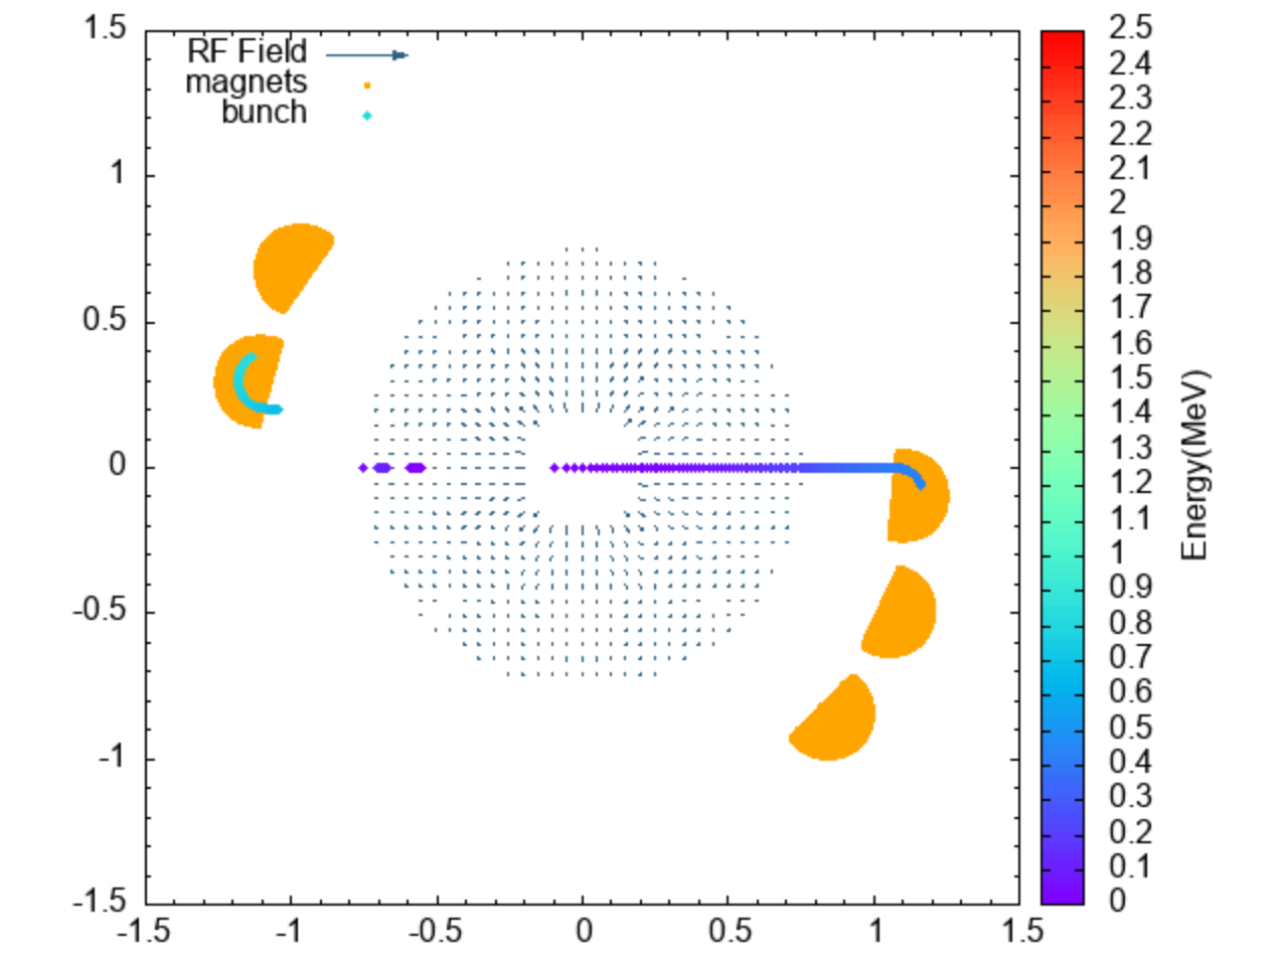
\includegraphics[width=\linewidth]{../../../figures/rhodoSim/5ns_gnuplot.png}
        \caption*{Unsyncronized \e gun period, $T_g = 5ns$}
    \end{subfigure}
    \begin{subfigure}{0.9\textwidth}
        \centering
        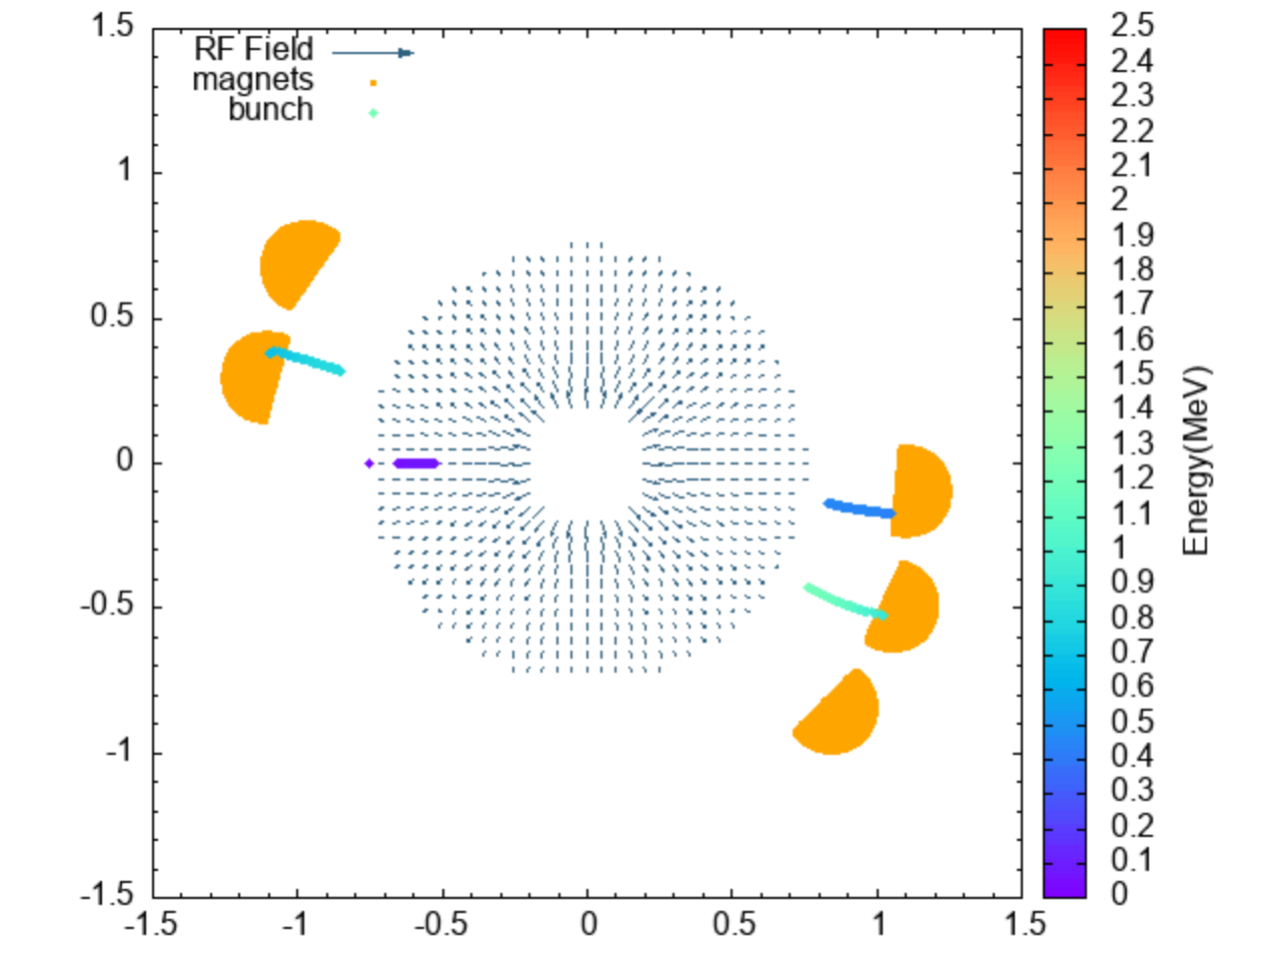
\includegraphics[width=\linewidth]{../../../figures/rhodoSim/9_3ns_gnuplot.png}
        \caption*{Syncronized \e gun period, $T_g = 9.3ns$}
    \end{subfigure}
    \caption{Example \textit{gnuplot} renders of \textit{Rhodotron Simulation}\\$P=12$kW, $f=107.5$MHz}
    \label{fig:example_gnuplot_renders}
\end{figure}

\subsection{Acceleration in Magnetic Field}
An issue regarding the \eB interaction became apparent when energy gain during these interactions was observed.
A setup simulation was implemented in which a bunch of 100\e at $1$MeV was fired to a uniform magnetic field of $0.1$T placed in $x>0.05$m.
Initial results at $dt=0.01$ns proved the suspicion of \eB interaction being broken. However, the energy gain would decrease tremendously as $dt$ decreased.


\begin{figure}[H]
    \captionsetup[subfigure]{justification=centering}
    \captionsetup{justification=centering}
    \centering
    \begin{subfigure}{0.8\textwidth}
        \centering
        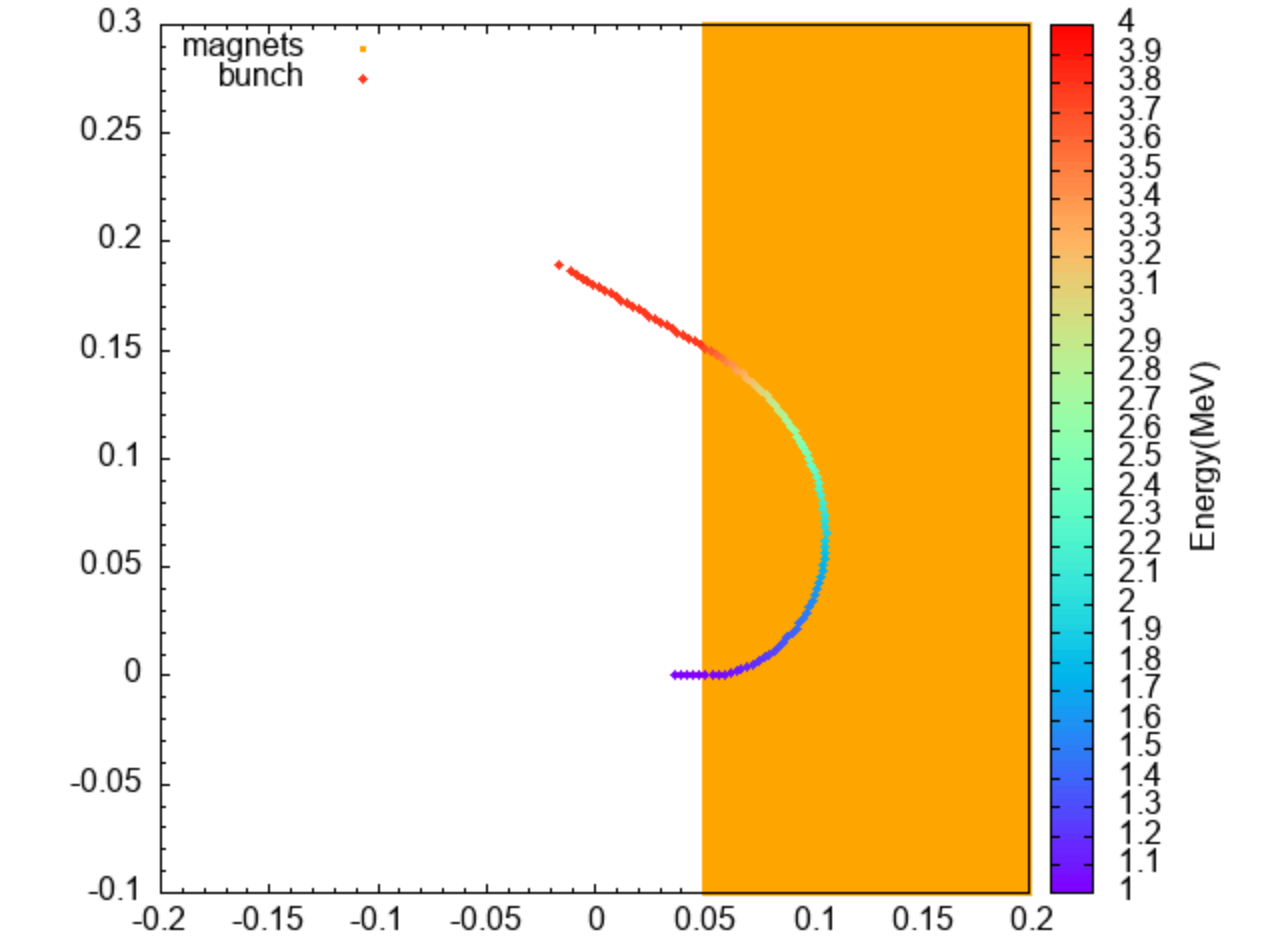
\includegraphics[width=\linewidth]{../../../figures/rhodoSim/mag_lf_001dt.png}
        \caption*{$dt=10^{-2}$ns, $\Delta E=2.783$MeV}
    \end{subfigure}
    \begin{subfigure}{0.8\textwidth}
        \centering
        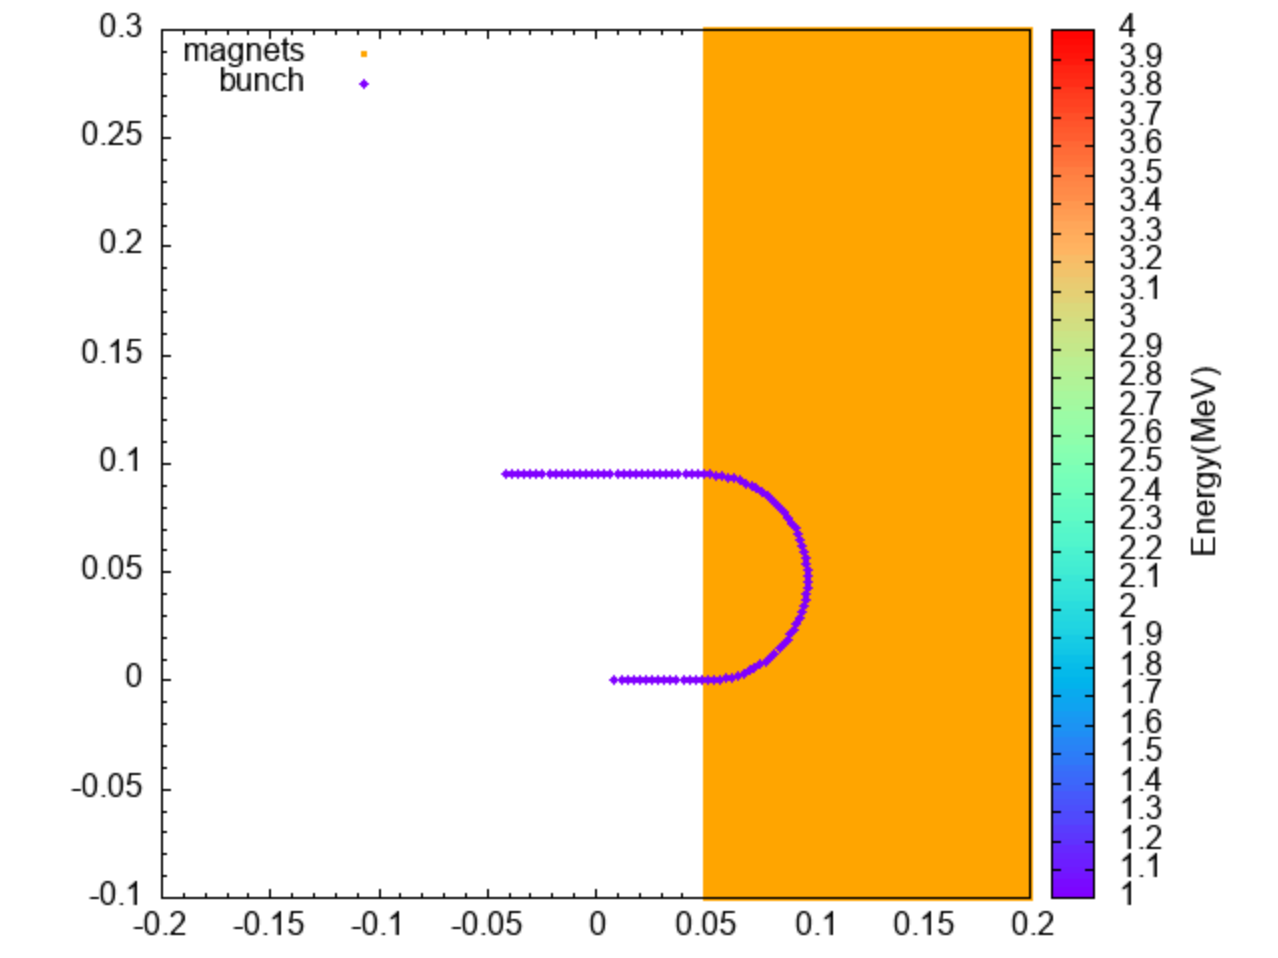
\includegraphics[width=\linewidth]{../../../figures/rhodoSim/mag_lf_00001dt.png}
        \caption*{$dt=10^{-4}$ns, $\Delta E=0.011$MeV}
    \end{subfigure}
    \caption{Energy gain of $1$MeV bunch in \textbf{B}=$0.1$T}
    \label{fig:mag_lf_render}
\end{figure}

Decreasing $dt$ would be the best way to increase accuracy of the results; however, this is not sustainable because time and computing power. 
Until this point, \textit{Rhodotron Simulation} have been using \fromsec{leapfrog} for \eEM interactions. 
To test newer approaches, two additional version of  \eEM interaction that are using \fromsec{rungekutta} were added.
\subsubsection{RK4-1}
First approach for integrating \fromsec{rungekutta} into \eEM interaction was to calculate $\vecthreeBF{a}_{E}$ and $\vecthreeBF{a}_{B}$ from \fromeq{acc_of_E_and_B} using \textit{RK4}.
After $\vecthreeBF{a}_{EM} = \vecthreeBF{a}_{E} + \vecthreeBF{a}_{B}$ was calculated, \e would move and accelerate using the \textit{Leap-frog} method. 
The idea was to produce more refined interaction results, leading to improved accuracy especially in \eB.
RF field was kept static during the RK4 computation, due to ongoing \textit{multithreading} implementation efforts. 
The implementation can be found in \fromfigs{rk1_B}{rk1_EM}.
\subsubsection{RK4-2}
Following the implementation of \textit{RK4-1}, revisions were made to the integration method for \textit{RK4} to replace \textit{Leap-frog}.
Instead of calculating $\vecthreeBF{a}_{EM}$ using \textit{RK4}, $\vecthreeBF{r}$ and $\vecthreeBF{v}$ would be determined directly.

These three methods were then tested in the same setup as \fromfig{mag_lf_render}. The results can be found in \fromfig{lf_rk1_rk2_comparison}.

\begin{figure}[H]
    \captionsetup[subfigure]{justification=centering}
    \captionsetup{justification=centering}
    \centering
    \begin{subfigure}{0.8\textwidth}
        \centering
        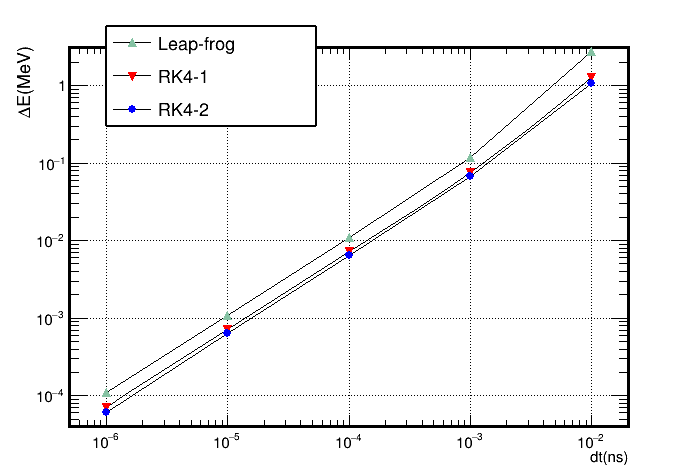
\includegraphics[width=\linewidth]{../../../figures/analiz/lf_rk1_rk2_dt-E.png}
        \caption*{$dt$ vs $\Delta E$}
    \end{subfigure}
    
    \begin{subfigure}{0.8\textwidth}
        \centering
        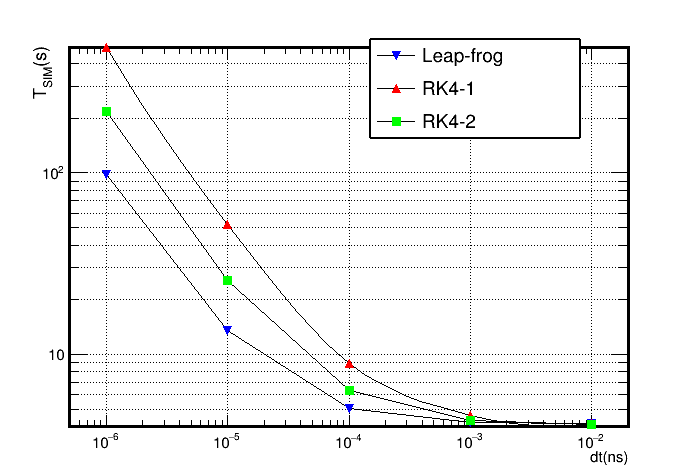
\includegraphics[width=\linewidth]{../../../figures/analiz/lf_rk1_rk2_dt-Tsim.png}
        \caption*{$dt$ vs $T_{sim}$}
    \end{subfigure}
    \caption{Comparing Leap-frog, RK4-1, RK4-2 performance on \eB interaction\\ $E_{in}=1$MeV, \textbf{B}=$0.1$T, $t_{end}=5$ns}
    \label{fig:lf_rk1_rk2_comparison}
\end{figure}

The data from these tests can be found in \fromtabs{lf_rk1_rk2_Tsim}{lf_rk1_rk2_dE} of \fromapp{example_simulation_runs}. 
As anticipated, \textit{Leap-frog} produced the fastest yet least accurate results, whereas \textit{RK4-2} method was proved to be the best performer for accuracy.
When $dt=10^-5$ns was taken as reference point due to providing a good balance of accuracy and computational intensity, 
\textit{RK4-2} provides around $41\%$ less energy gain in $\vecthreeBF{B}$ with respect to the next performer \textit{Leap-frog}.
The tradeoff is the computational intensity mentioned in \fromsec{rungekutta}; \textit{Leap-frog} being around $47\%$ faster than $\textit{RK4-2}$.

This relation is not linear however; \textit{RK4-2} is not as demanding in less computationally intensitive runs and able to keep up with \textit{Leap-frog} in execution times while increasing the accuracy difference from other methods,
whereas \textit{Leap-frog} excels at simplicity, being able to use higher time resolution for given computational power. 
Both methods can be used in different situations, therefore both were integrated into \textit{Rhodotron Simulation} for the user to decide.
\textit{RK4-2} renders from these test can be found in \fromfig{mag_rk_render} of \fromapp{example_simulation_runs}.



\subsection{Acceleration in Electric Field}
After the accuracy concerns regarding the \eB interaction were raised, it was decided to test \eE and compare the performance of \textit{Leap-frog} and \textit{RK4}.

As test setups, two simulation confgurations were made. They aimed to test the accuracy of acceleration of a beam in parallel and perpendicular static uniform electric fields.
Both configurations had an \egun located at $(-0.753, 0, 0)$m, directed at $(1, 0, 0)$ firing electrons with the kinetic energy of $1$MeV. 

\begin{figure}[H]
    \centering
    \begin{subfigure}{0.47\textwidth}
        \centering
        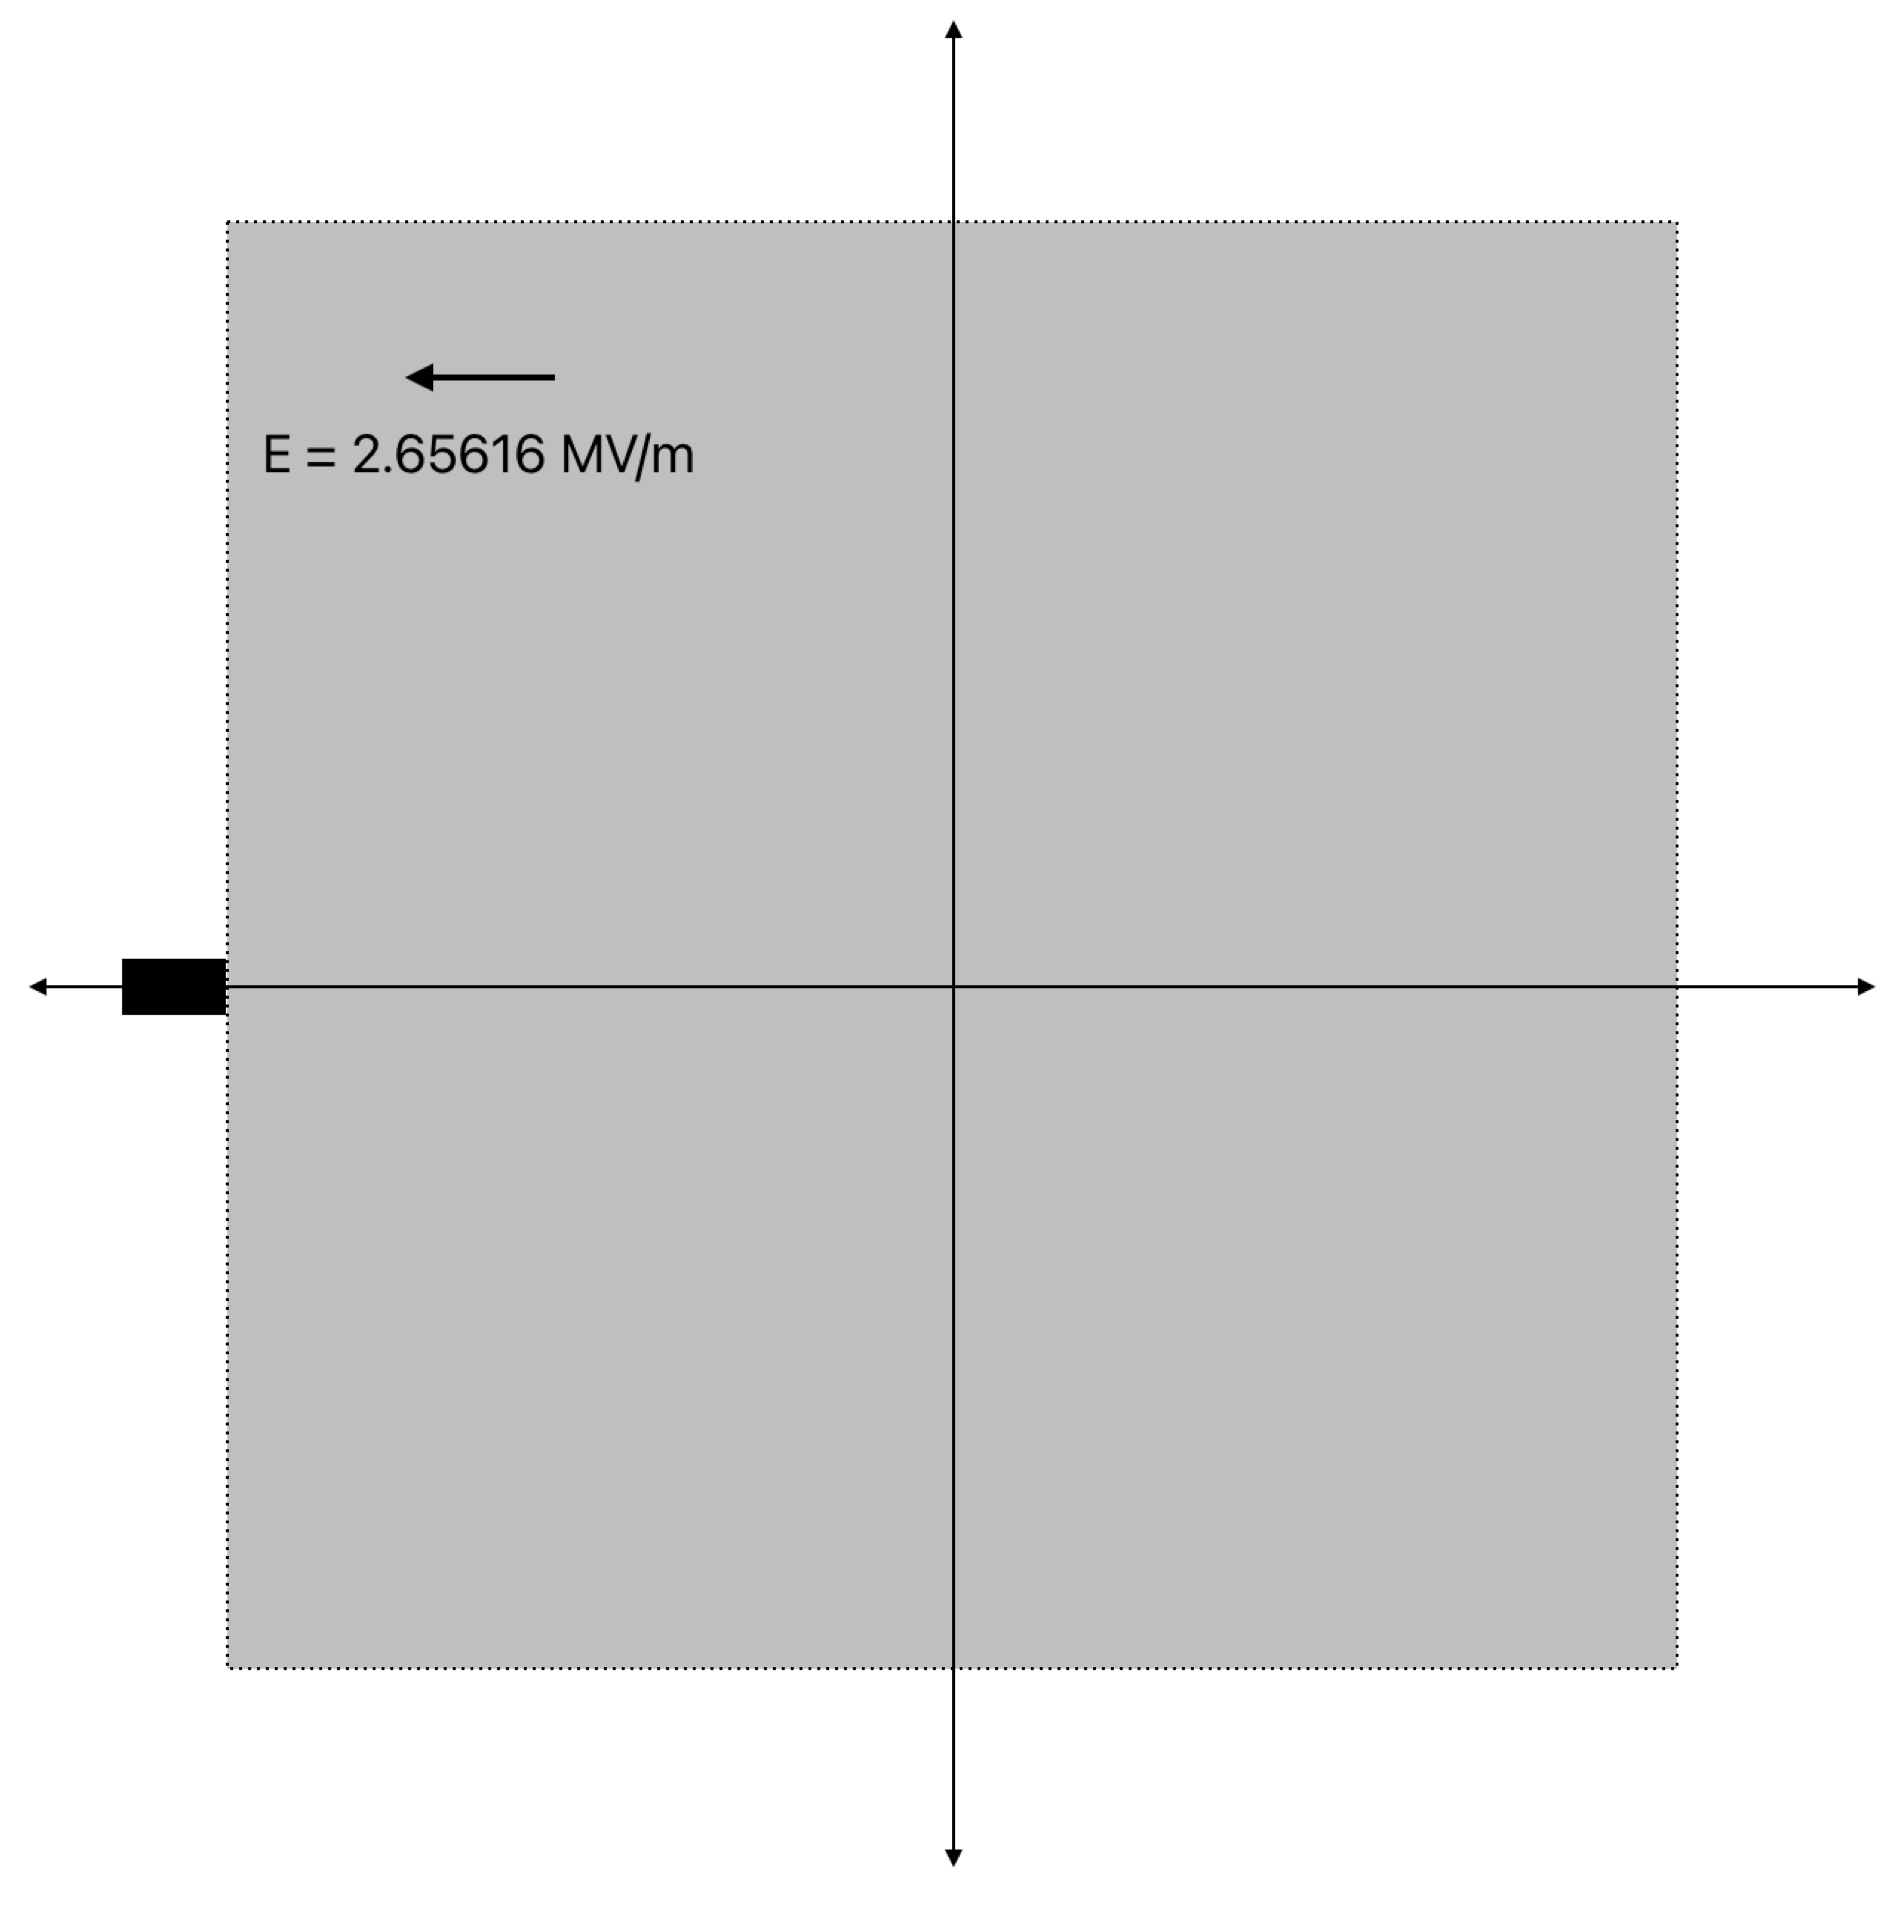
\includegraphics[width=0.9\linewidth]{../../../figures/illustrations/statE_1.png}
        \caption*{Setup-1 parallel $\vecthreeBF{E}$ field}
    \end{subfigure}
    \begin{subfigure}{0.48\textwidth}
        \centering
        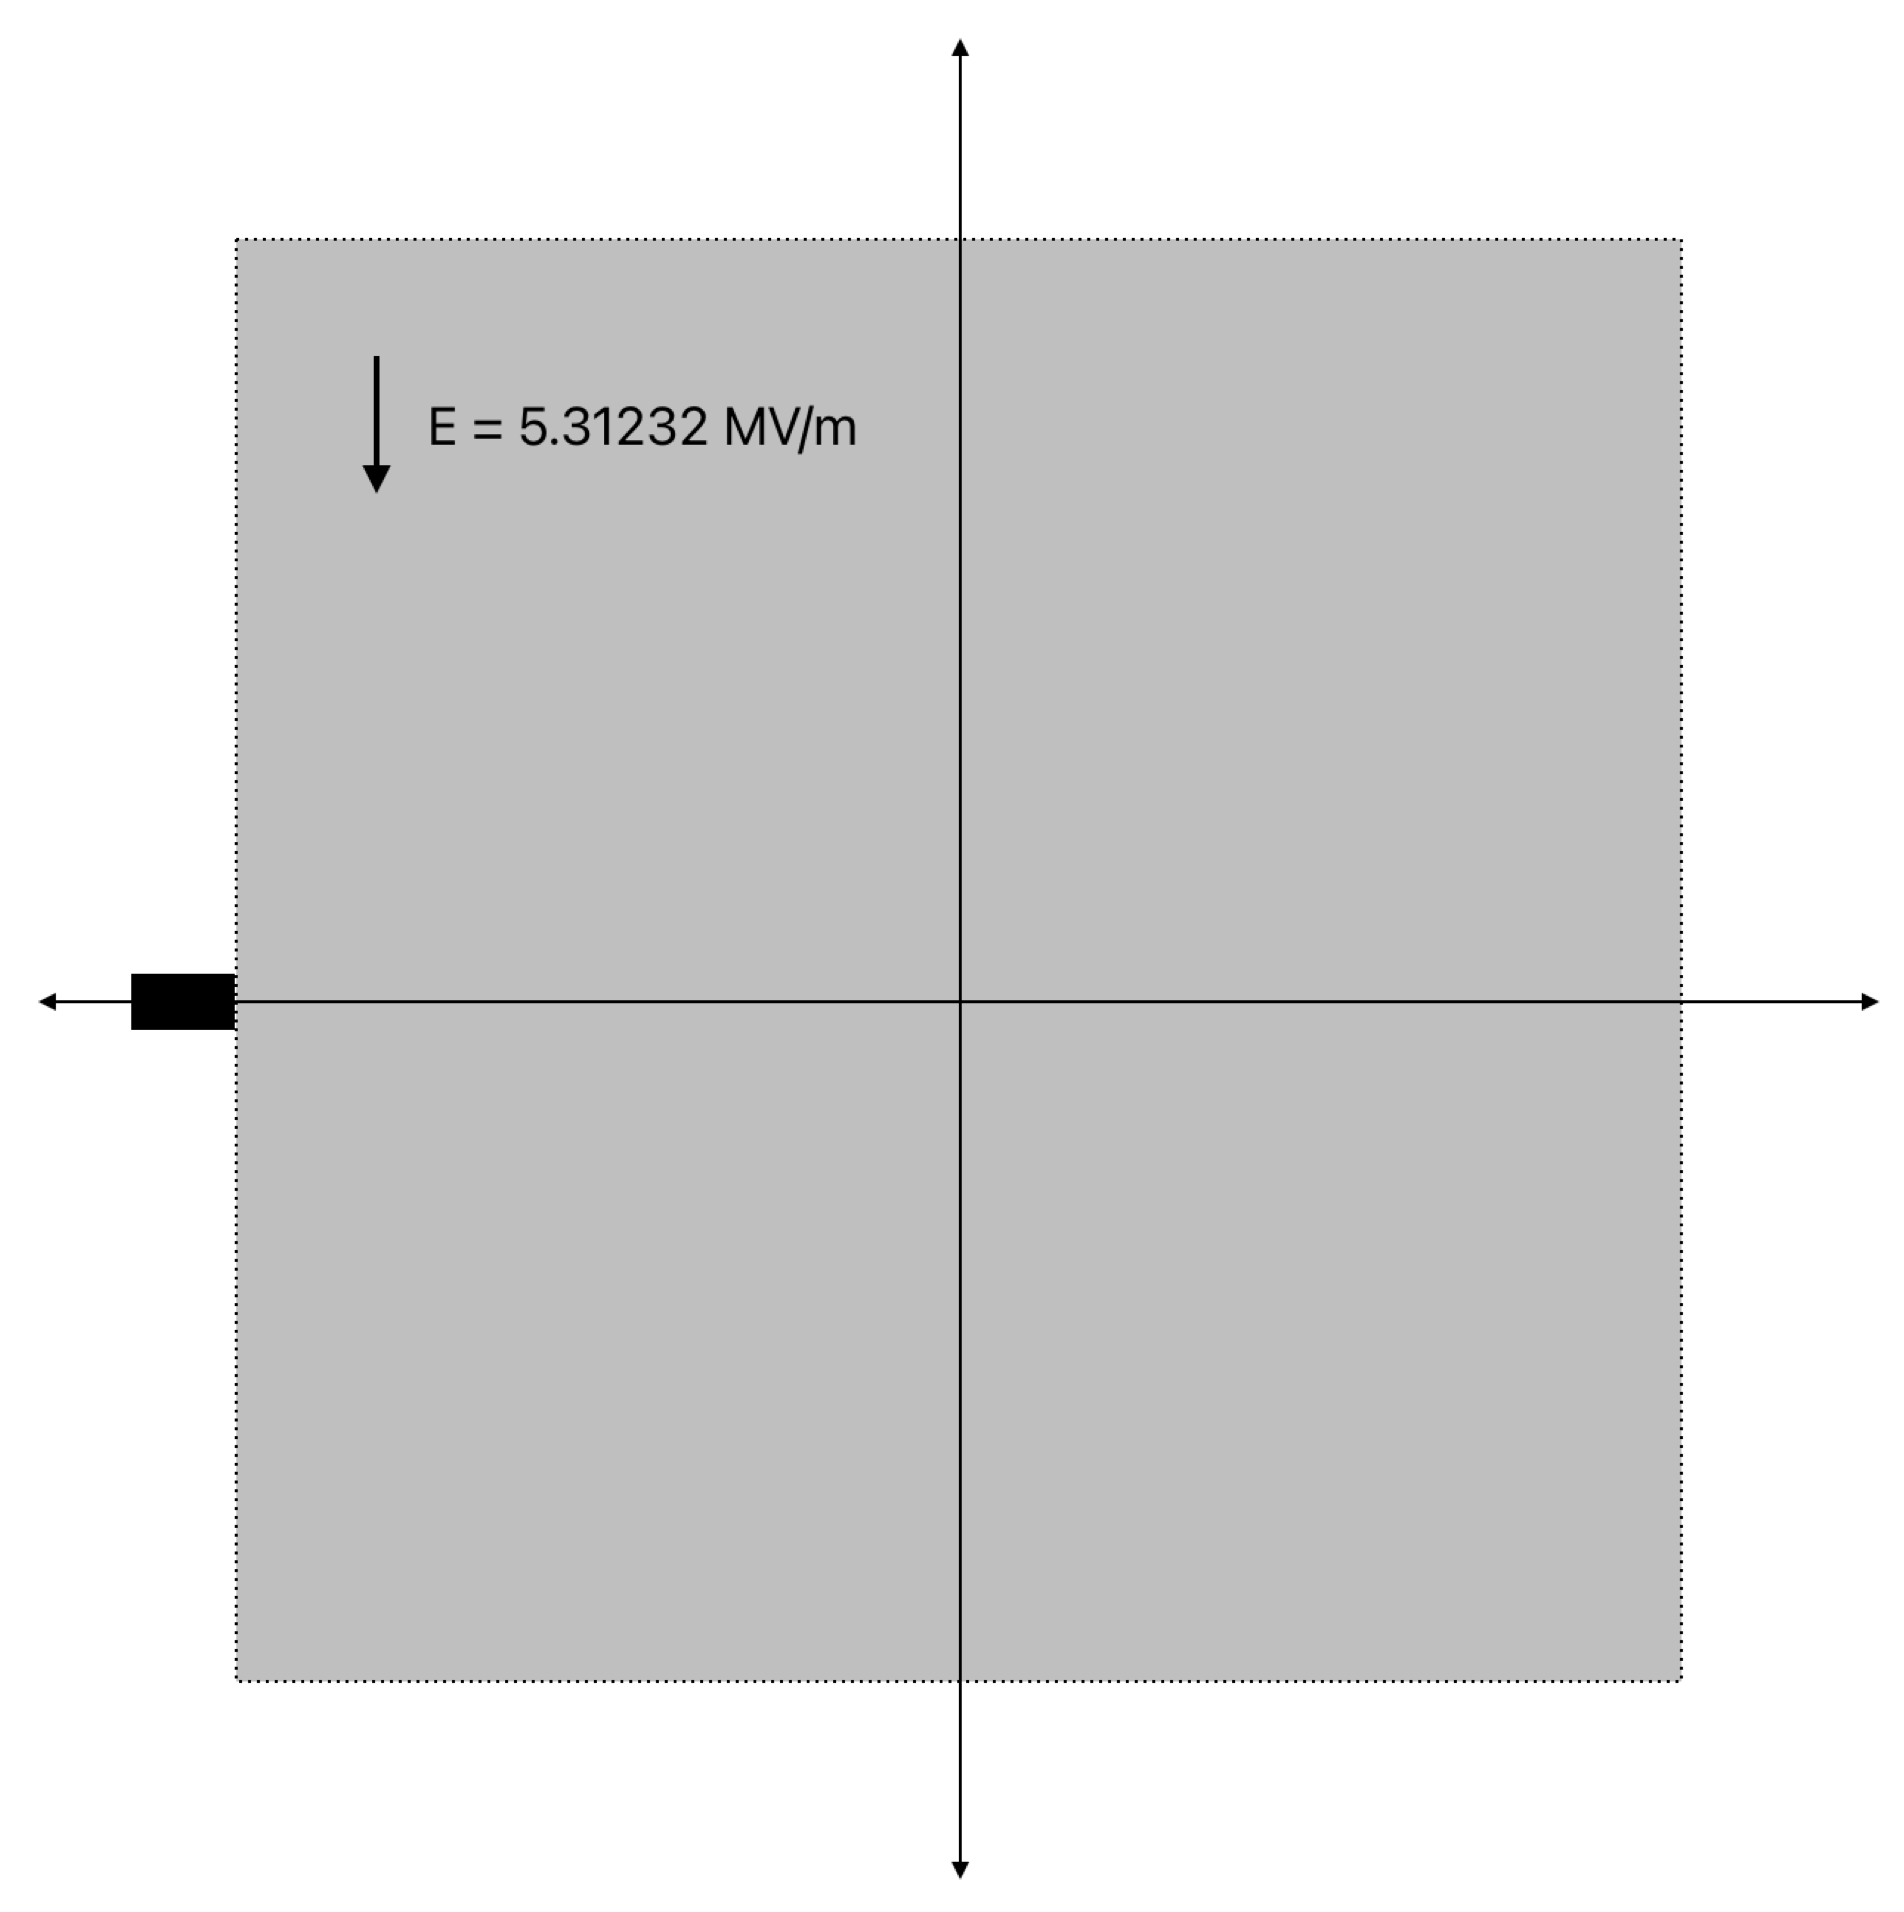
\includegraphics[width=0.9\linewidth]{../../../figures/illustrations/statE_2.png}
        \caption*{Setup-2, perpendicular $\vecthreeBF{E}$ field}
    \end{subfigure}
    \caption{Illustration of test setups.}
\end{figure}

In the first test, the beam would be injected into a static uniform electric field \\
$\vecthreeBF{E}=(-2.65616, 0, 0)$ MV/m where $-0.753<x<0.753$ and $-0.753<y<0.753$, $\vecthreeBF{E}=0$ elsewhere.

Considering the $\vecthreeBF{E}$ is parallel to the beam path, potential difference $V$ in the trejectory until \vecNum{-0.753, 0, 0} is
\begin{eqnarray}
    \Delta V^1 &=& - \int \dotProdBF{E}{ds} \\
             &=& - \int_{-0.753}^{0.753} -2.65616 \times dx \\
             &=& 2.65616 \times 1.506 \\
    \Delta V^1 &=& 4 MV \\
    \Delta E^1 &=& 4 MeV \\
    E_{exitTH}^1 &=& 5 MeV
\end{eqnarray}

In the second test on the other hand, the beam would be injected into a different static uniform electric field, \\
$\vecthreeBF{E}=(0, -5.31232, 0)$ MV/m where $-0.753<x<0.753$ and $-0.753<y<0.753$, $\vecthreeBF{E}=0$ elsewhere.
\begin{eqnarray}
    \Delta V^2   &=& - \int \dotProdBF{E}{ds} \\
                 &=& - \int_{0}^{0.753} -5.31232 \times dy \\
                 &=& 5.31232 \times 0.753 \\
    \Delta V^2   &=& 4 MV \\
    \Delta E^2   &=& 4 MeV \\
    E_{exitTH}^2 &=& 5 MeV
\end{eqnarray}

Therefore, in the both tests, the beam was expected to exit $\vecthreeBF{E}$ with $E_{exitTH} = 5$ MeV. 
To also measure the variance in simulation completion times, $T_{sim}$, set of $10$ runs were completed at the configuration for each $dt$ value.

\begin{figure}[H]
    \centering
    \begin{subfigure}{0.8\textwidth}
        \centering
        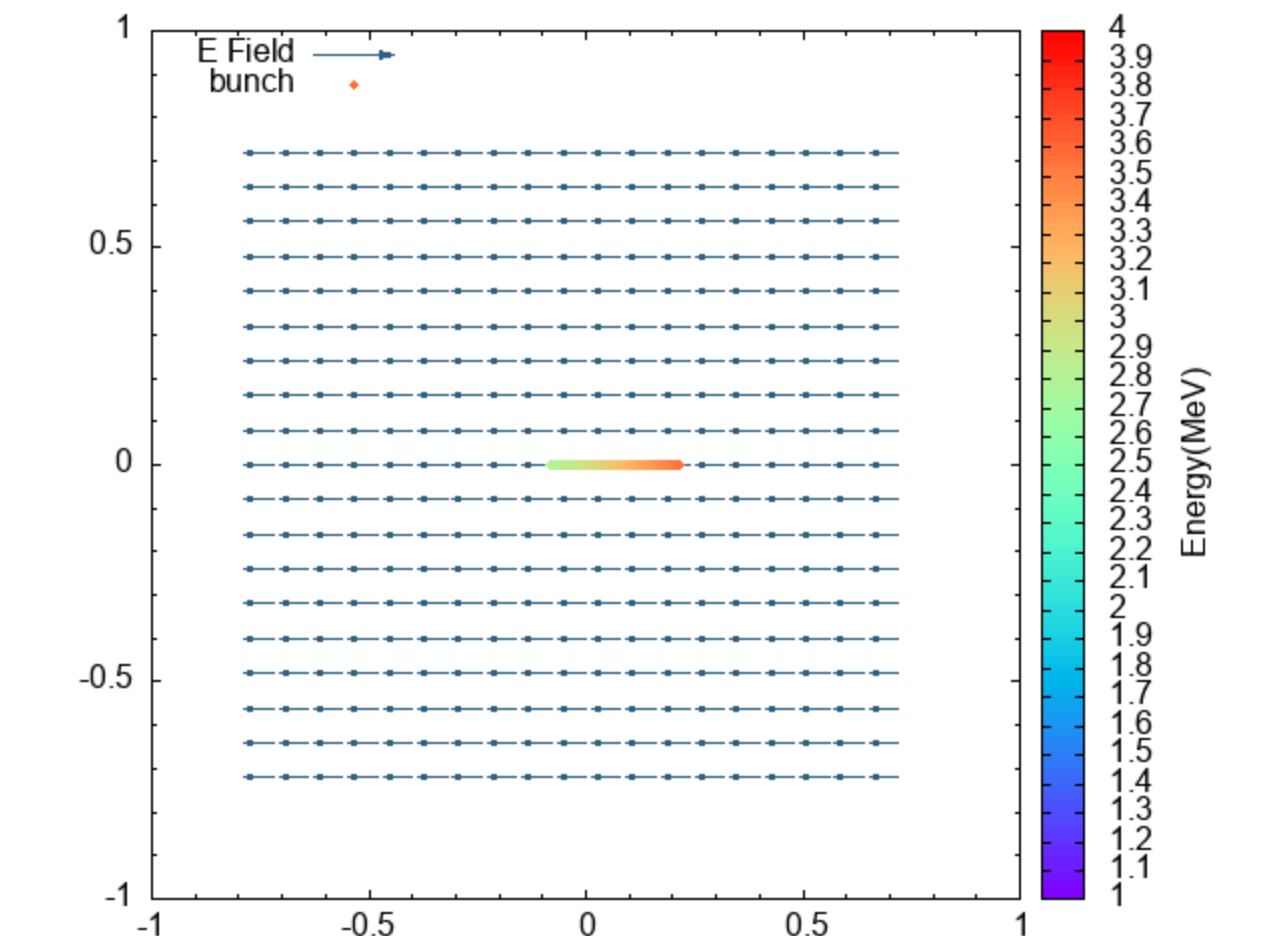
\includegraphics[width=\linewidth]{../../../figures/rhodoSim/statE_par.png}
        \caption*{Setup-1, $\textbf{V}_{\parallel}$=4MV}
    \end{subfigure}
    \begin{subfigure}{0.8\textwidth}
        \centering
        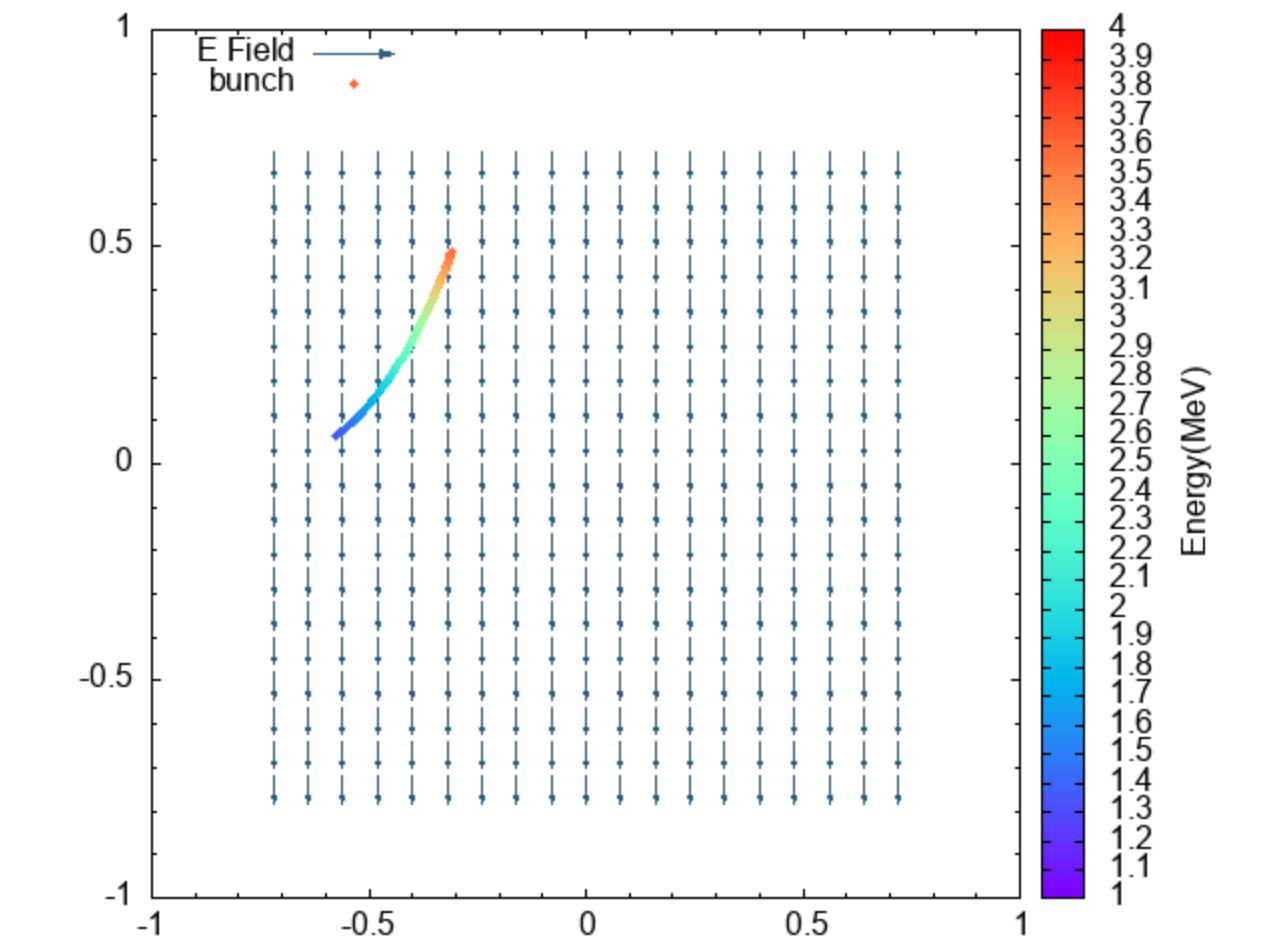
\includegraphics[width=\linewidth]{../../../figures/rhodoSim/statE_perp.png}
        \caption*{Setup-2, $\textbf{V}_{\perp}$=4MV}
    \end{subfigure}
    \caption{Render of the test setups. \\ $E_{in}=1$ MeV, $t_{end}=6$ns}
\end{figure}


\begin{figure}[H]
    \captionsetup[subfigure]{justification=centering}
    \captionsetup{justification=centering}
    \centering
    \begin{subfigure}{0.9\textwidth}
        \centering
        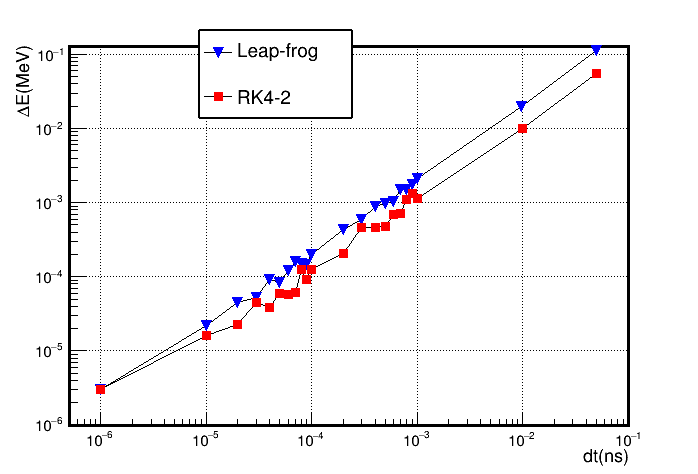
\includegraphics[width=\linewidth]{../../../figures/analiz/staticE_lf_rk2_dt-E.png}
        \caption*{$dt$ vs $\Delta E$}
    \end{subfigure}
    
    \begin{subfigure}{0.9\textwidth}
        \centering
        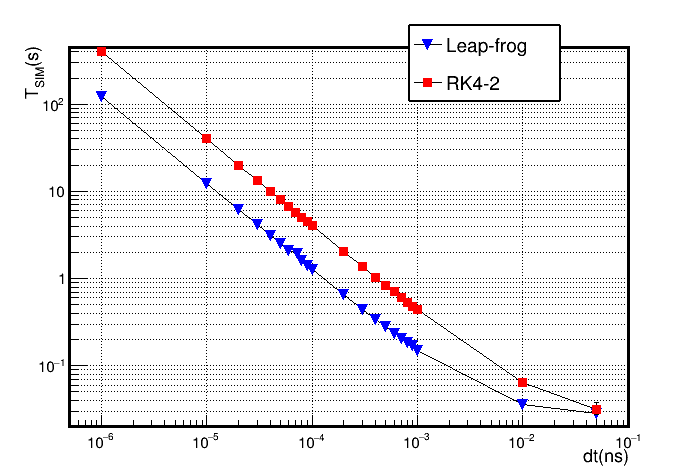
\includegraphics[width=\linewidth]{../../../figures/analiz/staticE_lf_rk2_dt-Tsim.png}
        \caption*{$dt$ vs $T_{sim}$}
    \end{subfigure}
    \caption{Comparing Leap-frog, RK4-2 performance on \eE interaction\\ $E_{in}=1$MeV, $\textbf{V}_{\parallel}$=4MV, $t_{end}=6$ns}
    \label{fig:lf_rk2_par_stat_E_comparison}
\end{figure}

\begin{figure}[H]
    \captionsetup[subfigure]{justification=centering}
    \captionsetup{justification=centering}
    \centering
    \begin{subfigure}{0.9\textwidth}
        \centering
        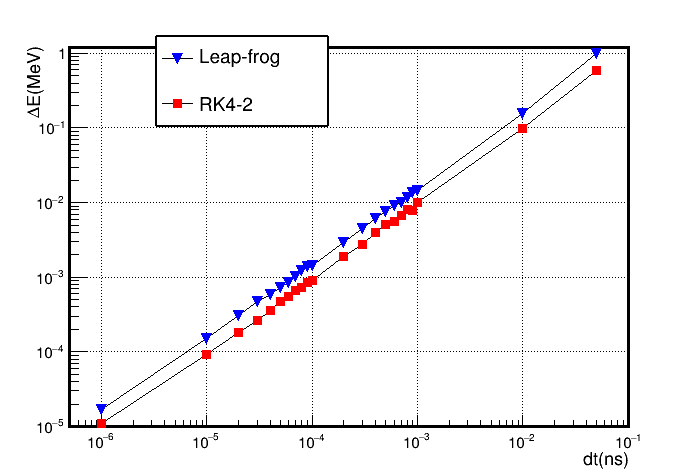
\includegraphics[width=\linewidth]{../../../figures/analiz/90staticE_lf_rk2_dt-E_3.png}
        \caption*{$dt$ vs $\Delta E$}
    \end{subfigure}
    
    \begin{subfigure}{0.9\textwidth}
        \centering
        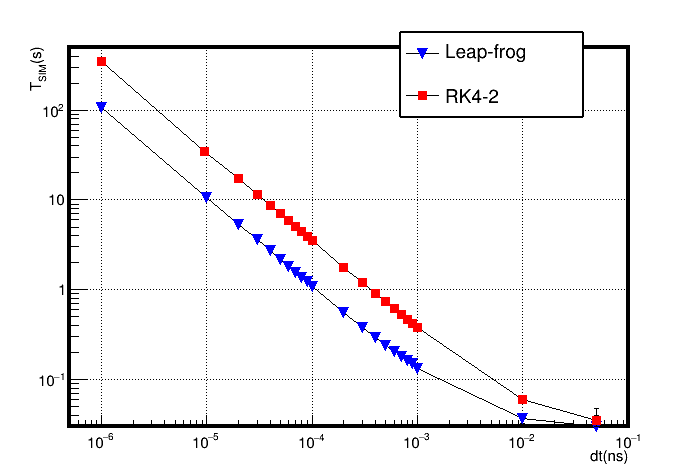
\includegraphics[width=\linewidth]{../../../figures/analiz/90staticE_lf_rk2_dt-Tsim.png}
        \caption*{$dt$ vs $T_{sim}$}
    \end{subfigure}
    \caption{Comparing Leap-frog, RK4-2 performance on \eE interaction\\ $E_{in}=1$MeV, $\textbf{V}_{\perp}$=4MV, $t_{end}=6$ns}
    \label{fig:lf_rk2_perp_stat_E_comparison}
\end{figure}



\subsection{Multithreading}
As already mentioned before, multithreading implementation efforts were ongoing since right after the start of this project. 
There have been a number of different approaches for implementation. 
First implemenation was done when the \textit{Rhodotron Simulation} was only capable of 1D simulations.
After the sizable refactoring done for 3D capabilities, this implementation was obselete. 

\begin{figure}[H]
    \centering
    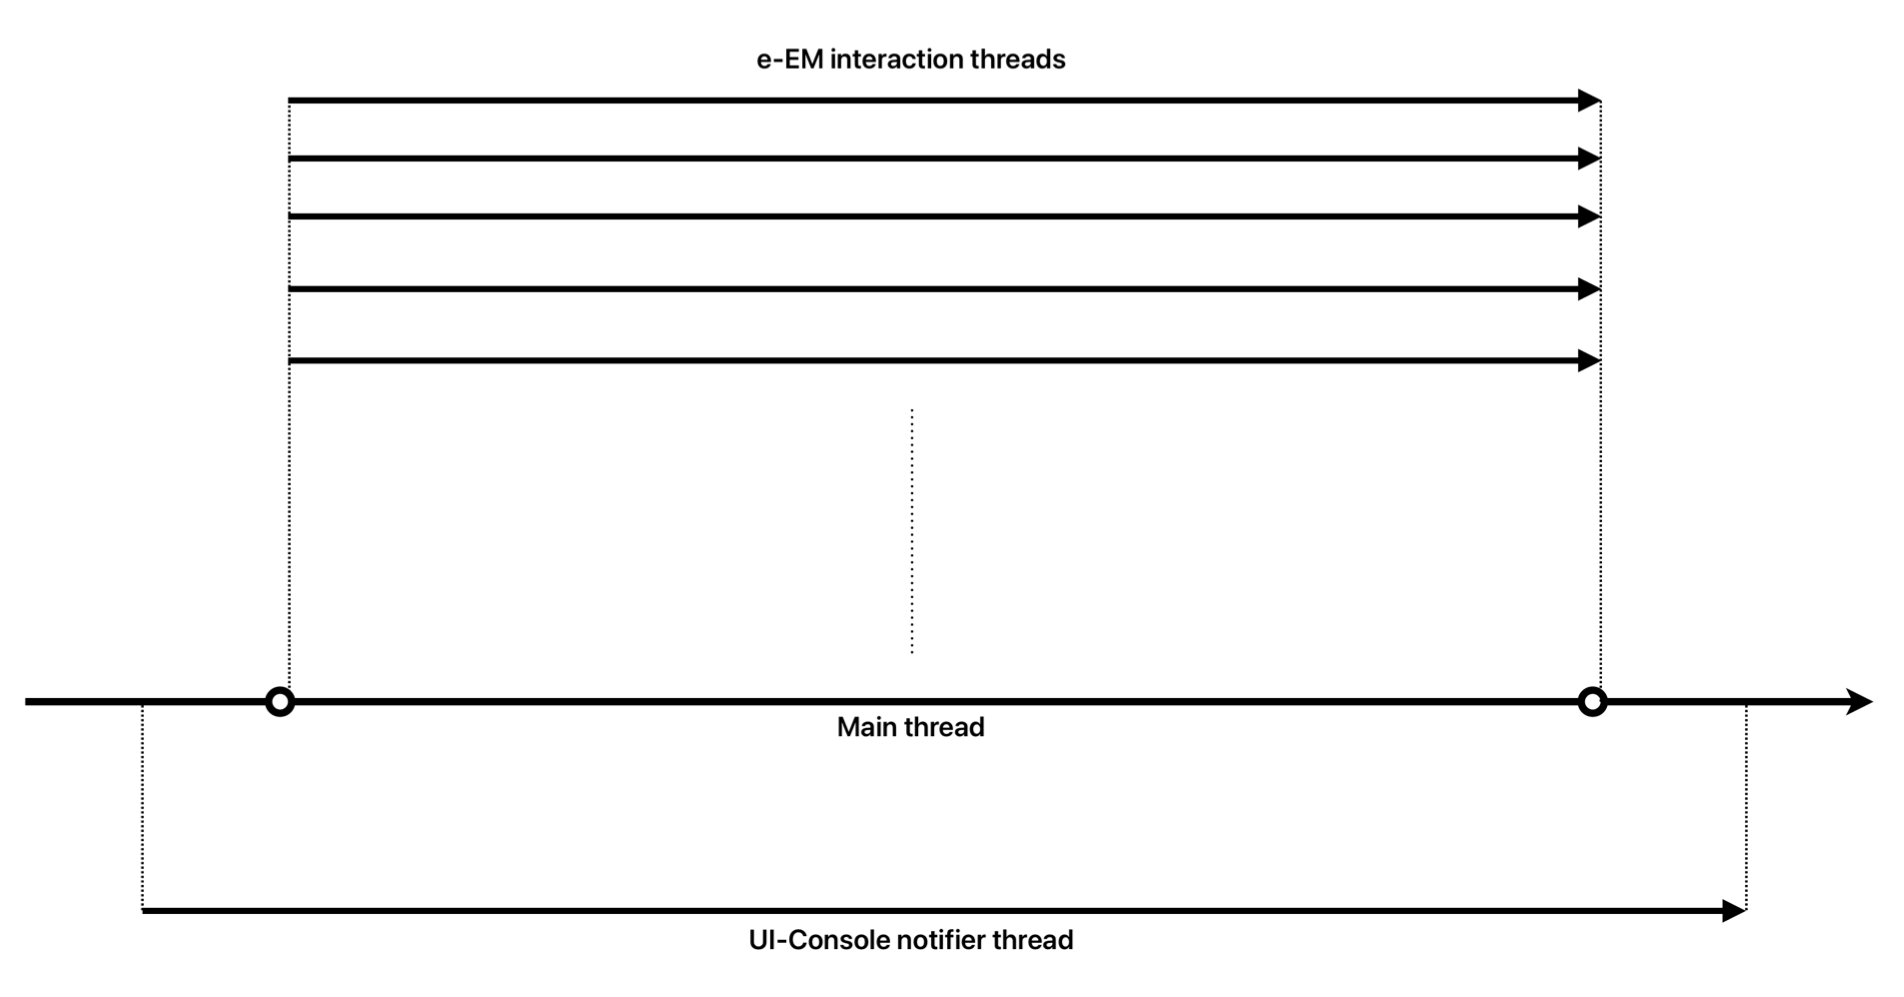
\includegraphics[width=\linewidth]{../../../figures/illustrations/multh_arc.png}
    \caption{An Illustration of the multithreading architecture.}
    \label{fig:multh_illustration}
\end{figure}

For the current version, a main thread that spawns and manages several other worker threads would be used as can be seen in \fromfig{multh_illustration}.
The UI-Console thread would handle incoming and outgoing communication, notifying the user about the status of simulation (see \fromfig{console_output_running} in \fromapp{console_output_running}) 
or communucating with the \textit{GUI} that will be disscussed in the next section.

Focus of this section is the worker threads, also known as \eEM interaction threads.
There were four competing architecture for these worker threads,
\begin{enumerate}
    \item Have a thread pool that calculates \eEM in a queue 
    \item Assign a thread to each bunch
    \item Assign random electrons to each thread and calculate \eEM with global time
    \item Assign random electrons to each thread and calculate \eEM with local thread time
\end{enumerate}

\textbf{Architecture 1} would require constant waiting in worker threads to get mutexes of $\vecthreeBF{E}$ field, especially in \textit{RK4}.

\textbf{Architecture 2} was performing well in configurations with a large number of bunches, but was not increasing performance in lower bunch count configurations as expected.

\textbf{Architecture 3} was inefficient and wasteful since all the worker threads would wait the main thread to get the next time after they finish calculation, while the main thread would be waiting for the slowest worker thread.

\textbf{Architecture 4} was thought to be the best performer. It would give freedom to calculate the whole simulation to each thread while giving up the global time.
This would also mean thread-safety is ensured since there is no shared data between the worker threads. 
However, this architecture can cause issues if \ee interactions were decided to be implemented in the future.

Another caveat is that a copy operation of $\vecthreeBF{E}$ and $\vecthreeBF{B}$ objects for each worker thread would be needed.
This would lead to larger memory allocations and more time spent setting up simulations. 
Therefore, \textit{Architecture 4} is not ideal for fast calculations and when the memory is an important constraint.
An implementation that can use both \textbf{Architecture 2} \& \textbf{Architecture 4} when necessary would be a better approach considering these methods;
nevertheless, \textbf{Architecture 4} was chosed to be implemented.





\subsection{Graphical User Interface}
Until this point, \textit{Rhodotron Simulation} could be used with a configration file, defining the problem that would be simulated.
An example of this configuration file can be found in \fromfig{config_file} of \fromapp{example_simulation_runs}. 
This approach was simple and fast; however, it was not suitable for the average target user since required basic knowledge of command line interface and was not up to modern standards.
For this reason, a GUI was decided to be built, using \textit{ROOT framework}. 
This would also enable \textit{Rhodotron simulation} to make use of analysis tools offered by \textit{ROOT}.

The initial design of the \textit{Rhodotron Simulation GUI} can be observed in \fromfig{gui_illustration}.

\begin{figure}[H]
    \centering
    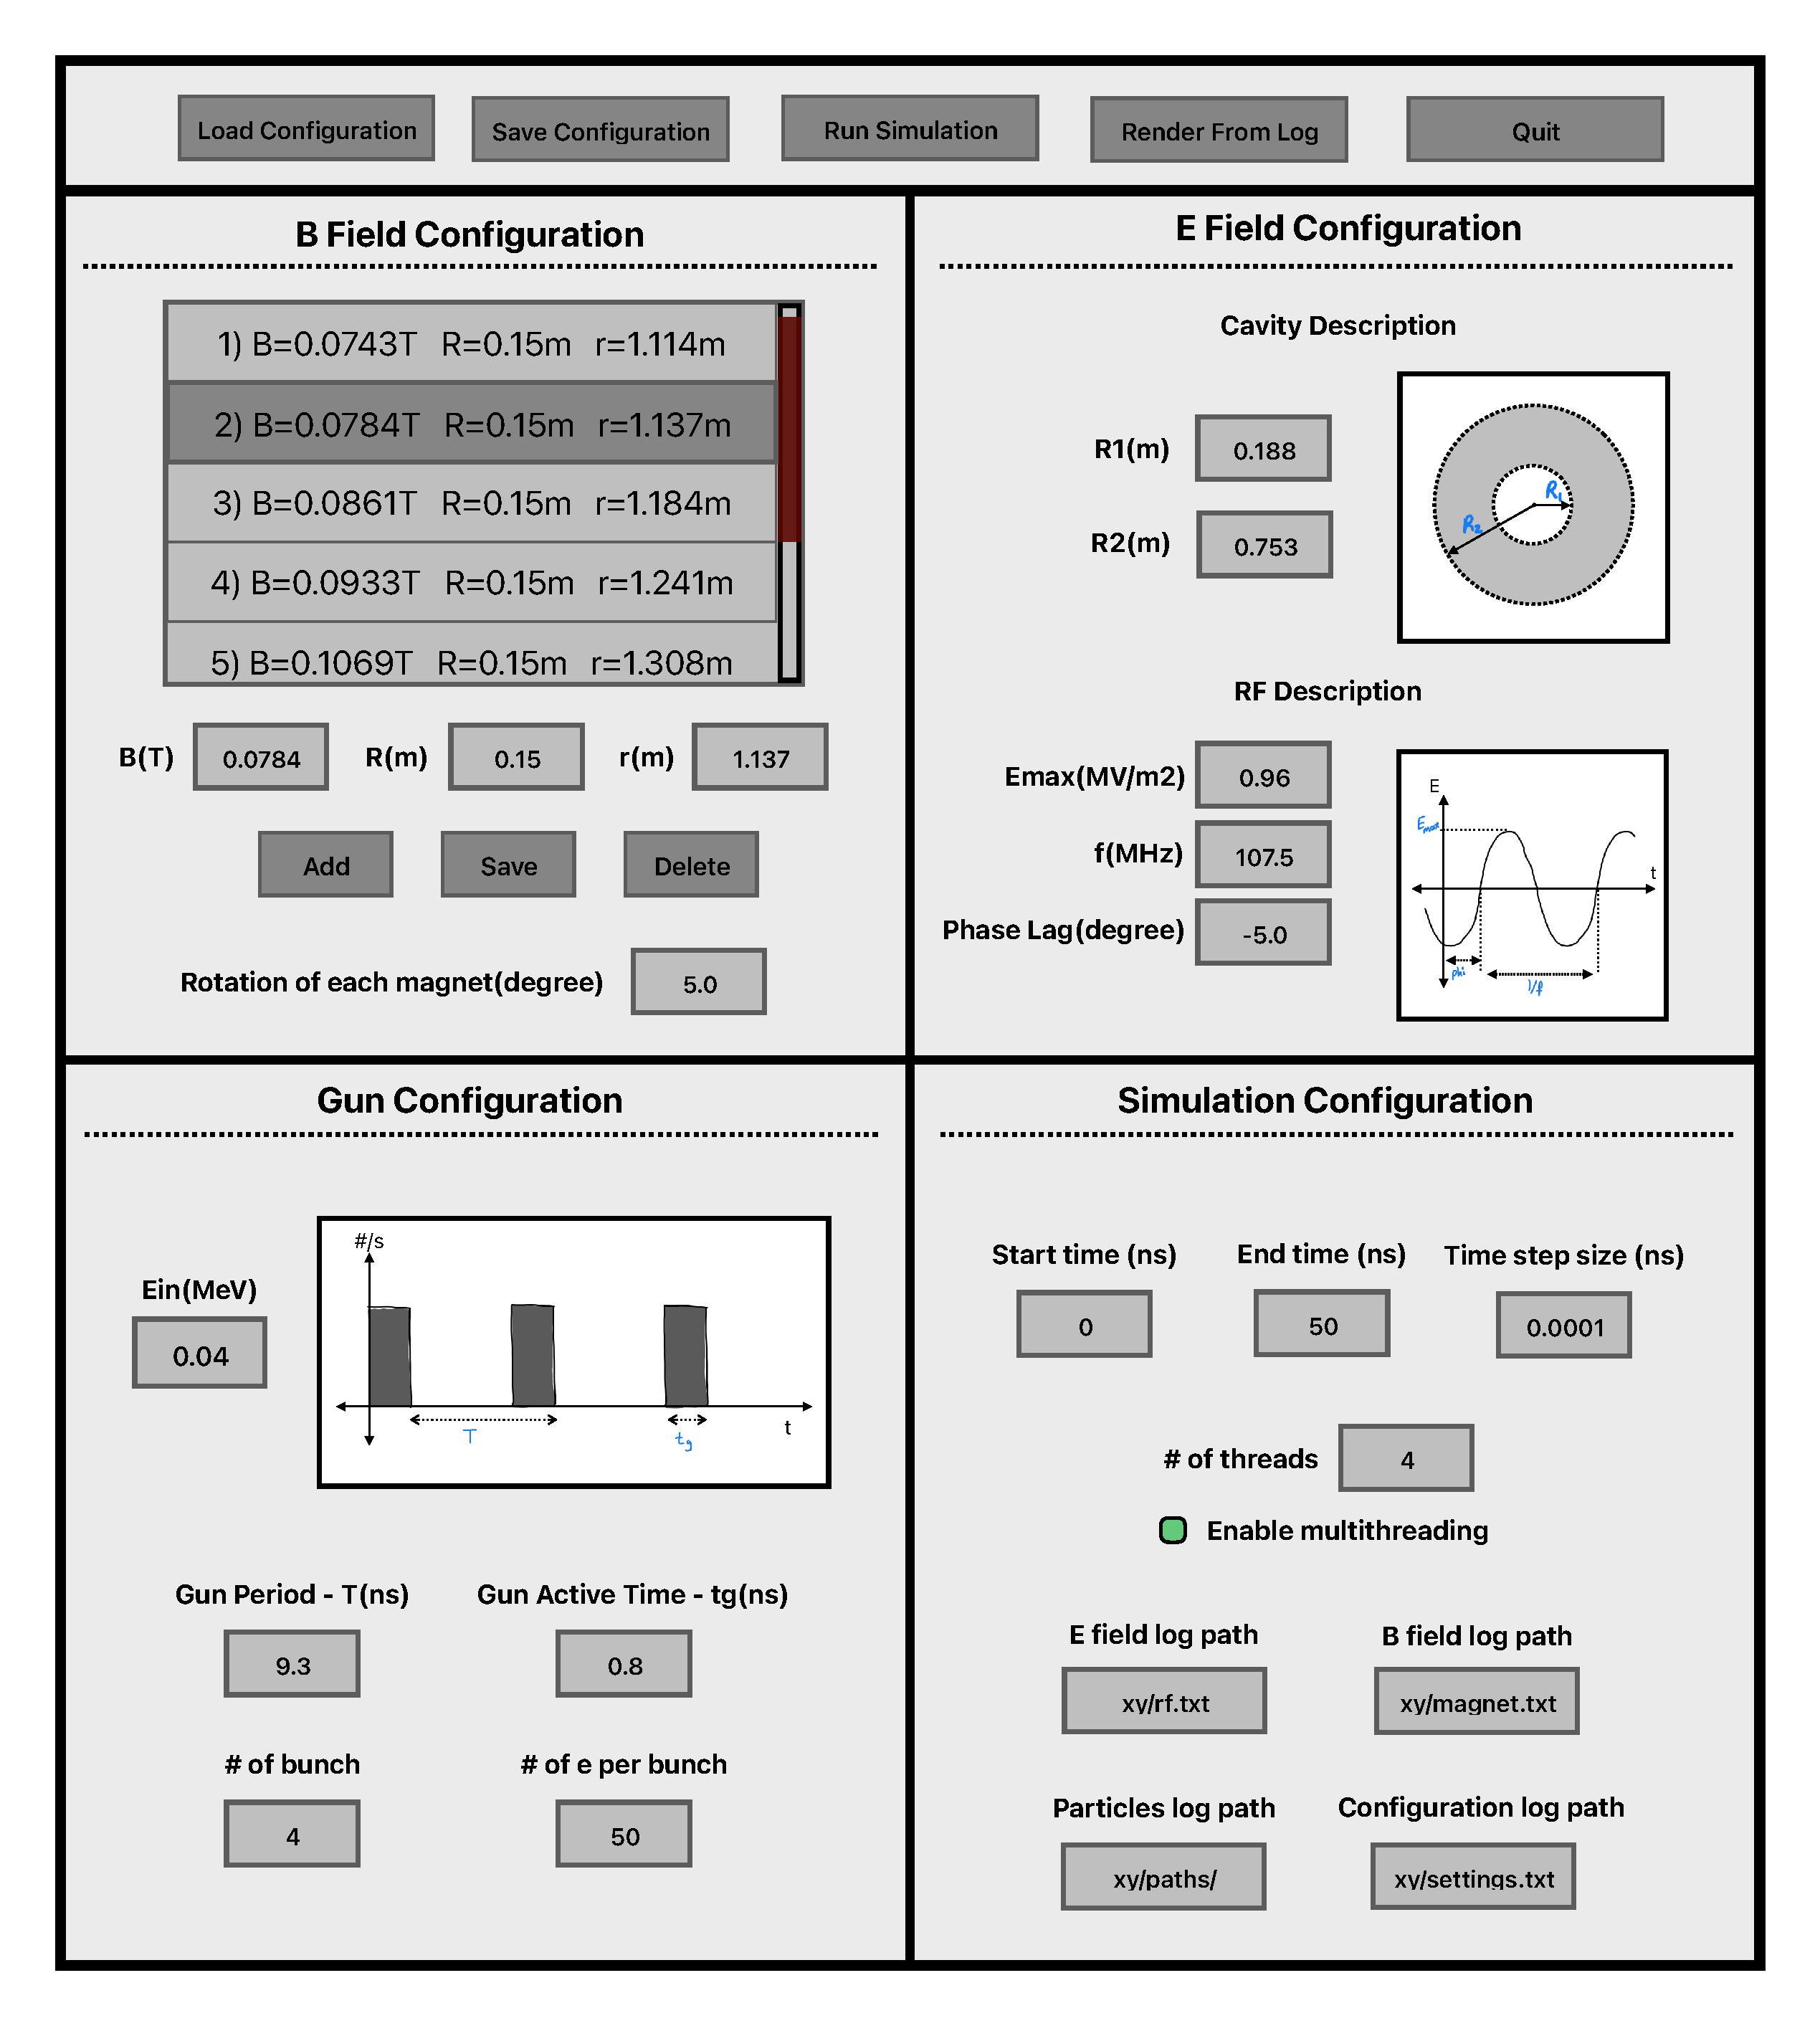
\includegraphics[width=\linewidth]{../../../figures/illustrations/RhodoSim_GUI_Draft_V02.pdf}
    \caption{An Illustration of first GUI design.}
    \label{fig:gui_illustration}
\end{figure}

The \textit{GUI} would be a standalone application, running the \textit{Rhodotron Simulation} as a service when needed. 
For this reason, the now called \textit{simulation engine} was updated to be able to run as a background service of \textit{GUI}.
By this approach, one could also ignore the \textit{GUI} altogether and use the \textit{simulation engine} as before, as these are two seperate products.




%%%%%%


\appendix
\chapter{Intermediate Codes} \label{appendix:intermediate_codes}
\begin{figure}[H]
    \centering
    \captionsetup{justification=centering}
    \begin{subfigure}{\textwidth}
        \centering
        \begin{minted}[linenos=true, autogobble, frame=lines, framesep=2mm, fontsize=\scriptsize]{c++}
            for(double i = 2; i < 9; i += dT_out){
                t_dum += i;
                double enow = gecis(r_pos, vel, Et, t_dum);
                if( enow > maxE ){
                  maxE = enow;
                  t_opt = i;
                }
                t_dum = t;
            }
        \end{minted}
    \end{subfigure} 
    \\
    \begin{subfigure}{\textwidth}
        \centering
        \begin{minted}[linenos=true, autogobble, frame=lines, framesep=2mm,  fontsize=\scriptsize]{c++}
            double gecis(double r_pos, double vel, double Et, double &t){
                for(; r_pos >= -R2 && r_pos <= R2 ; t+=dT){
                    vel = c*sqrt(Et*Et-E0*E0)/Et;
                    double RelBeta  = vel/c;
                    double RelGamma = 1.0 / sqrt(1.0-RelBeta*RelBeta);
                
                    double ef=Eradial(r_pos*1000,t,RFphase*deg_to_rad);
                
                    double acc=ef*1E6*eQMratio/(RelGamma*RelGamma*RelGamma); 
                
                    r_pos = r_pos + vel * dT*ns + 1/2*acc*(dT*ns)*(dT*ns);
                    vel=vel+acc*dT*ns;
                    RelBeta  = vel/c;
                    RelGamma = 1.0 / sqrt(1.0-RelBeta*RelBeta);
                    Et=RelGamma*E0; 
                }
                return Et;
            }
        \end{minted}
    \end{subfigure}
    \caption{$L_{out}$ Optimization For Single \e}
    \label{fig:lout_opt_single_e}
\end{figure}

\begin{figure}[H]
        \centering
        \captionsetup{justification=centering}
        \begin{minted}[linenos=true, autogobble, frame=lines, framesep=2mm, fontsize=\scriptsize]{c++}
            int phase_opt(const vector<double>& Louts, int phase_sweep_range){
                double minrms = 1;
                int opt_phase;
                for(int RFphase = -phase_sweep_range; RFphase <= phase_sweep_range; RFphase++){
                    Bunch bunch1(RFphase);
                    double t1 = 0;
                    bunch1.bunch_gecis_t(t1);
                    bunch1.reset_pos();
            
                    for(int i = 0; i < Louts.size(); i++){
                        bunch1.bunch_gecis_d(Louts[i]);
                        bunch1.reset_pos();
                    }
                        
                    if( bunch1.E_rms() < minrms ){
                        minrms = bunch1.E_rms();
                        opt_phase = RFphase;
                    }
                }
                return opt_phase;
            }
        \end{minted}
    \caption{$\phi_{lag}$ Optimization For Initial Bunch Design}
    \label{fig:phlag_opt_n_pass}
\end{figure}

\begin{figure}[H]
    \captionsetup[subfigure]{justification=centering}
    \captionsetup{justification=centering}
    \begin{subfigure}{\textwidth}
        \begin{minted}[linenos=true, autogobble, frame=lines, framesep=2mm, fontsize=\scriptsize]{c++}
            double vector3d::operator* (const vector3d& other){
                double dot = 0;
                dot += this->x * other.x;
                dot += this->y * other.y;
                dot += this->z * other.z;
                return dot;
            }
        \end{minted}
    \end{subfigure}

    \begin{subfigure}{\textwidth}
        \begin{minted}[linenos=true, autogobble, frame=lines, framesep=2mm, fontsize=\scriptsize]{c++}
            vector3d vector3d::operator% (const vector3d& other){
                double x_ = (this->y * other.z) - (this->z * other.y);
                double y_ = (this->z * other.x) - (this->x * other.z);
                double z_ = (this->x * other.y) - (this->y * other.x);
                vector3d crossed(x_, y_, z_);
                return crossed;
            }
        \end{minted}
    \end{subfigure}
    \caption{* and \% operators of \textit{vector3d} class}
    \label{fig:vector3d_dot_cross_product}
\end{figure}

\begin{figure}[H]
    \centering
    \captionsetup{justification=centering}
    \begin{minted}[linenos=true, autogobble, frame=lines, framesep=2mm, fontsize=\scriptsize]{c++}
        bool isInsideHalfSphere(vector3d e_position, double r, vector3d hs_position){
            vector3d relative = e_position - hs_position;       
            // r/5 can be changed, use this for now                                
            if ( relative.magnitude() <= r && relative * hs_position.direction() >= -r/5){      
                return true;                                                                 
            }
            return false;
        }
    \end{minted}
\caption{Logic of is \e inside the shape of magnet}
\label{fig:is_inside_halfsphere}
\end{figure}

\begin{figure}[H]
    \centering
    \captionsetup{justification=centering}
    \begin{minted}[linenos=true, autogobble, frame=lines, framesep=2mm, fontsize=\scriptsize]{c++}
        vector3d Electron2D::interactB_RK(const MagneticField& B, double time_interval){
            if (B.isInside(pos) == -1){
                return vector3d(0,0,0);
            }
            Electron2D e_dummy;
            e_dummy.Et = Et;
            e_dummy.pos = pos;
            e_dummy.vel = vel;
            double time_halved = time_interval*0.5;
            // get k1                                       
            vector3d F_m = (e_dummy.vel % B.getField(pos))*eQMratio;                                       
            vector3d k1 = F_m * e_dummy.gamma_inv();     
            // get k2
            e_dummy.move(time_halved);
            e_dummy.accelerate(k1, time_halved);                                              
            F_m = (e_dummy.vel % B.getField(pos))*eQMratio;                                               
            vector3d k2 = F_m * e_dummy.gamma_inv();    
            // get k3
            e_dummy.vel = vel;
            e_dummy.accelerate(k2, time_halved);
            vector3d k3 = F_m * e_dummy.gamma_inv();   
            // get k4
            e_dummy.vel = vel;
            e_dummy.move(time_halved);
            e_dummy.accelerate(k3, time_interval);                                           
            F_m = (e_dummy.vel % B.getField(pos))*eQMratio;  
            vector3d k4 = F_m * e_dummy.gamma_inv();
        
            return (k1 + k2*2 + k3*2 + k4)/6;
        }
    \end{minted}
\caption{RK4-1 implemenation of \e-$\vecthreeBF{B}$}
\label{fig:rk1_B}
\end{figure}
\begin{figure}[H]
    \centering
    \captionsetup{justification=centering}
    \begin{minted}[linenos=true, autogobble, frame=lines, framesep=2mm, fontsize=\scriptsize]{c++}
        void Electron2D::interactRK_ActorE(const RFField& E, const MagneticField& B, double time_interval){
            vector3d run_kut_E = interactE_RK(E, time_interval);
            vector3d run_kut_B = interactB_RK(B, time_interval);
        
            vector3d acc = run_kut_E + run_kut_B;
            
            move(acc, time_interval/2);
            accelerate(acc, time_interval);
            move(acc, time_interval/2);
        }
    \end{minted}
\caption{RK4-1 implemenation of \eEM}
\label{fig:rk1_EM}
\end{figure}

\begin{figure}[H]
    \centering
    \captionsetup{justification=centering}
    \begin{minted}[linenos=true, autogobble, frame=lines, framesep=2mm, fontsize=\tiny]{c++}
        void Electron2D::interactRK(RFField& E, MagneticField& B, const double time, double time_interval){
            Electron2D e_dummy;
            e_dummy.Et = Et;
            e_dummy.pos = pos;
            e_dummy.vel = vel;
    
            // Calculate k1
            vector3d acc_E = E.actOn(e_dummy);
            vector3d acc_B = B.actOn(e_dummy);
            vector3d acc = acc_E + acc_B;
            e_dummy.move(time_interval);
            e_dummy.accelerate(acc, time_interval);
            vector3d pos_k1 = e_dummy.pos, vel_k1 = e_dummy.vel;
    
            // Calculate k2
            e_dummy.pos = (pos + pos_k1)*0.5;
            e_dummy.vel = (vel + vel_k1)*0.5;
            e_dummy.Et = e_dummy.gamma()*E0;
            E.update(time + time_interval*0.5);
    
            acc_E = E.actOn(e_dummy);
            acc_B = B.actOn(e_dummy);
            acc = acc_E + acc_B;
            e_dummy.move(time_interval);
            e_dummy.accelerate(acc, time_interval);
            vector3d pos_k2 = e_dummy.pos, vel_k2 = e_dummy.vel;
    
            // Calculate k3
            e_dummy.pos = (pos + pos_k2)*0.5;
            e_dummy.vel = (vel + vel_k2)*0.5;
            e_dummy.Et = e_dummy.gamma()*E0;
            E.update(time + time_interval*0.5);

            acc_E = E.actOn(e_dummy);
            acc_B = B.actOn(e_dummy);
            acc = acc_E + acc_B;
            e_dummy.move(time_interval);
            e_dummy.accelerate(acc, time_interval);
            vector3d pos_k3 = e_dummy.pos, vel_k3 = e_dummy.vel;
    
            // Calculate k4
            E.update(time + time_interval);

            acc_E = E.actOn(e_dummy);
            acc_B = B.actOn(e_dummy);
            acc = acc_E + acc_B;
            e_dummy.move(time_interval);
            e_dummy.accelerate(acc, time_interval);
            vector3d pos_k4 = e_dummy.pos, vel_k4 = e_dummy.vel;
    
            E.update(time);
            pos = (pos_k1 + pos_k2*2 + pos_k3*2 + pos_k4)/6;
            vel = (vel_k1 + vel_k2*2 + vel_k3*2 + vel_k4)/6;
            Et = gamma()*E0;
    }
    \end{minted}
\caption{RK4-2 implemenation of \eEM}
\label{fig:rk2_EM}
\end{figure}


\chapter{Example Simulation Runs} \label{appendix:example_simulation_runs}

\begin{figure}[H]
    \centering
    \captionsetup{justification=centering}
    \begin{minted}[linenos=true, autogobble, frame=lines, framesep=2mm, fontsize=\scriptsize, style=staroffice]{c++}
        Optimal phase with the least RMS : -5

        Simulation settings : 
        ph = -5 deg, gt = 1 ns, enum = 1000
        dT = 0.001 ns, dT_out = 0.01 ns
        
        For the 1th magnet:
        Optimum out path = 0.81044 m
        Magnet guide = 0.25852 m
        Rho = 0.088477 m
        Drift time of the first electron in the bunch : 7.688 ns
        Drift time of the last electron in the bunch : 7.487 ns
        Max energy = 0.47581 MeV
        RMS = 0.0058165 MeV
        
        For the 2th magnet:
        Optimum out path = 1.0833 m
        Magnet guide = 0.37766 m
        Rho = 0.098898 m
        Drift time of the first electron in the bunch : 5.597 ns
        Drift time of the last electron in the bunch : 5.617 ns
        Max energy = 0.89172 MeV
        RMS = 0.0099018 MeV
        
        For the 3th magnet:
        Optimum out path = 1.1705 m
        Magnet guide = 0.41573 m
        Rho = 0.10223 m
        Drift time of the first electron in the bunch : 5.314 ns
        Drift time of the last electron in the bunch : 5.325 ns
        Max energy = 1.298 MeV
        RMS = 0.013879 MeV

        Electron with the most energy : 623) 1.6999 MeV,	RMS of bunch : 0.017981 MeV
        
        Total steps calculated : 12468052652
        Simulation finished in : 632050015 us     ( 632.1 s )
        
    \end{minted}
\caption{$\phi_{lag}$, $\rho$ \& $L$ optimization at \\$P=12$KW, $R_1=0.188$m, $R_2=0.753$m, $t_g=1$ns, $E_{in}=40$KeV}
\label{fig:lout_opt_1ns_Erms}
\end{figure}

\begin{figure}[H]
    \centering
    \captionsetup{justification=centering}
    \begin{minted}[linenos=true, autogobble, frame=lines, framesep=2mm, fontsize=\scriptsize, style=staroffice]{c++}
        Optimal phase with the least RMS : 0

        Simulation settings : 
        ph = 0 deg, gt = 0.8 ns, enum = 1000
        dT = 0.001 ns, dT_out = 0.01 ns
        
        For the 1th magnet:
        Optimum out path = 0.80787 m
        Magnet guide = 0.2574 m
        Rho = 0.088379 m
        Drift time of the first electron in the bunch : 7.629 ns
        Drift time of the last electron in the bunch : 7.48 ns
        Max energy = 0.47579 MeV
        RMS = 0.0038689 MeV
        
        For the 2th magnet:
        Optimum out path = 1.0833 m
        Magnet guide = 0.37765 m
        Rho = 0.098898 m
        Drift time of the first electron in the bunch : 5.589 ns
        Drift time of the last electron in the bunch : 5.605 ns
        Max energy = 0.89169 MeV
        RMS = 0.0068848 MeV
        
        For the 3th magnet:
        Optimum out path = 1.1705 m
        Magnet guide = 0.41573 m
        Rho = 0.10223 m
        Drift time of the first electron in the bunch : 5.311 ns
        Drift time of the last electron in the bunch : 5.318 ns
        Max energy = 1.298 MeV
        RMS = 0.0096887 MeV
        
        Electron with the most energy : 629) 1.6999 MeV,	RMS of bunch : 0.012318 MeV
        
        Total steps calculated : 12455378454
        Simulation finished in : 631136046 us     ( 631.1 s )        
    \end{minted}
\caption{$\phi_{lag}$ \& $\rho$ \& $L$ optimization at \\$P=12$KW, $R_1=0.188$m, $R_2=0.753$m, $t_g=0.8$ns, $E_{in}=40$KeV}
\label{fig:lout_opt_08ns_Erms}
\end{figure}

\begin{table}[H]
    \centering
    \begin{tabular}{|l|l|l|l|l|l|l|l|l|l|}
    \hline
        $dt$(ns) & $T_{sim LF}(s)$ & $T_{sim RK1}(s)$  & $T_{sim RK2}(s)$  & $\Delta T_{LF-RK2}$\\\hline
        $10^{-2}$ & 4.14092 & 4.146 & 4.10945 & 0.77\% \\ \hline
        $10^{-3}$ & 4.23817 & 4.61703 & 4.30225 & -1.51\% \\ \hline
        $10^{-4}$ & 5.04679 & 8.93529 & 6.3065 & -24.96\% \\ \hline
        $10^{-5}$ & 13.5135 & 51.9024 & 25.4279 & -88.17\%\\ \hline
        $10^{-6}$ & 97.6229 & 486.378 & 217.704 & -123.01\% \\ \hline
    \end{tabular}
    \caption{$dt$ vs $T_{sim}$ of Leap-frog, RK4-1, RK4-2 \\$E_{in}=1$MeV, \textbf{B}=$0.1$T, $t_{end}=5$ns}
    \label{tab:lf_rk1_rk2_Tsim}
\end{table}

\begin{table}[H]
    \centering
    \begin{tabular}{|l|l|l|l|l|l|l|l|l|l|}
    \hline
        $dt$(ns) & $\Delta E_{LF}$(MeV) & $\Delta E_{RK1}$(MeV)  & $\Delta E_{RK2}$(MeV)  & $\Delta E_{LF-RK2}$\\\hline
        $10^{-2}$ & 2.78323 & 1.26503 & 1.04713 & 165.8\% \\ \hline
        $10^{-3}$ & 0.11712 & 0.07469 & 0.06691 & 42.87\% \\ \hline
        $10^{-4}$ & 0.01101 & 0.00716 & 0.00644 & 41.5\%  \\ \hline
        $10^{-5}$ & 0.00109 & 0.00071 & 0.00064 & 41\% \\ \hline
        $10^{-6}$ & 0.00011 & 0.00007 & 0.00006 & 45\% \\\hline
    \end{tabular}
    \caption{$dt$ vs $\Delta E$ of Leap-frog, RK4-1, RK4-2 \\$E_{in}=1$MeV, \textbf{B}=$0.1$T, $t_{end}=5$ns}
    \label{tab:lf_rk1_rk2_dE}
\end{table}

\begin{figure}[H]
    \captionsetup[subfigure]{justification=centering}
    \captionsetup{justification=centering}
    \begin{subfigure}{0.48\textwidth}
        \centering
        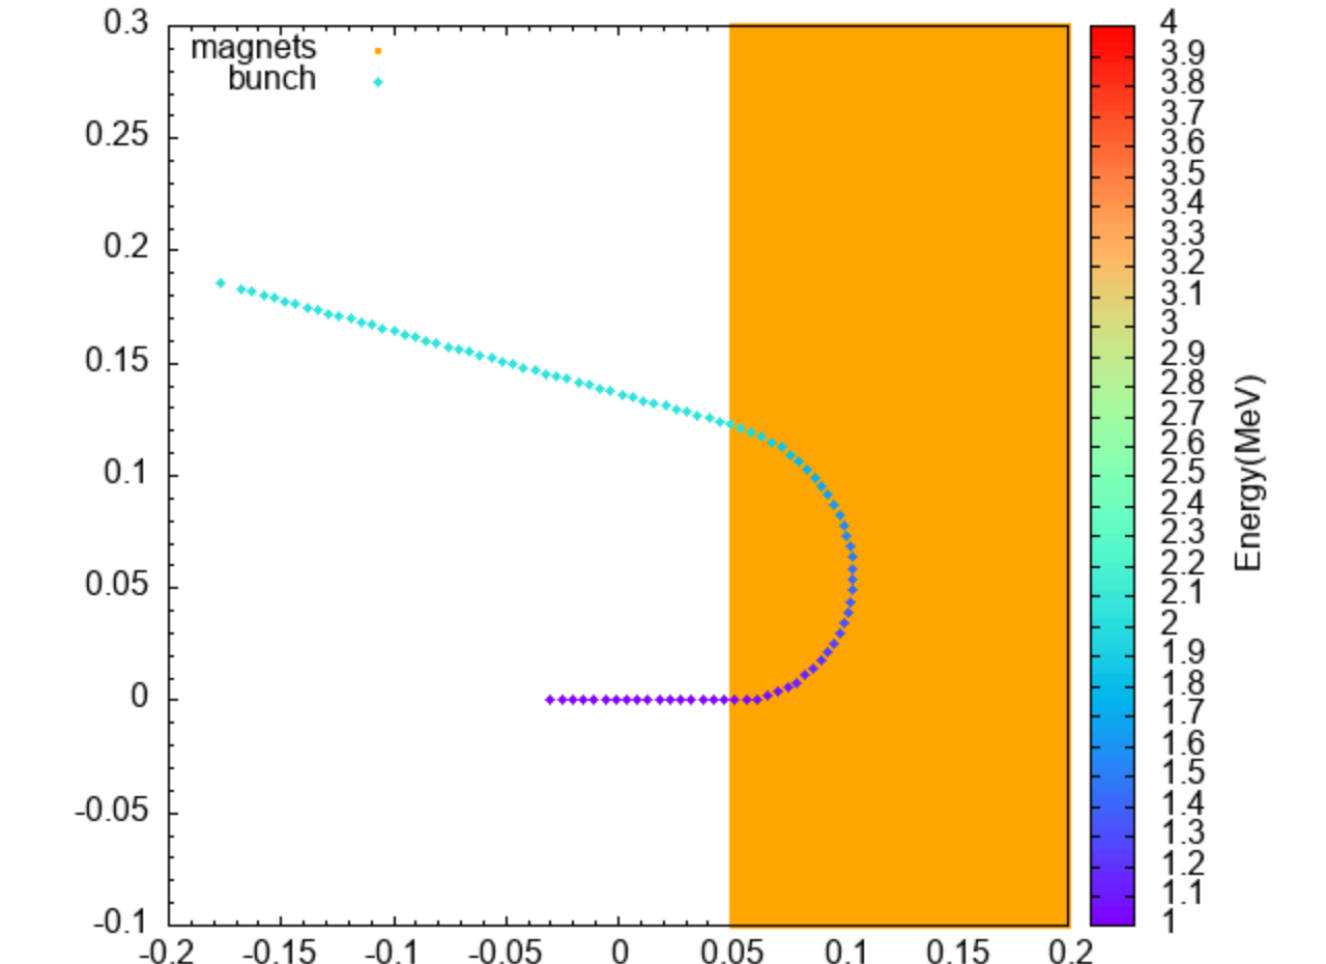
\includegraphics[width=\linewidth]{../../../figures/rhodoSim/mag_rk_001dt.png}
        \caption*{$dt=10^{-2}$ns, $\Delta E=1.047$MeV}
    \end{subfigure}
    \begin{subfigure}{0.48\textwidth}
        \centering
        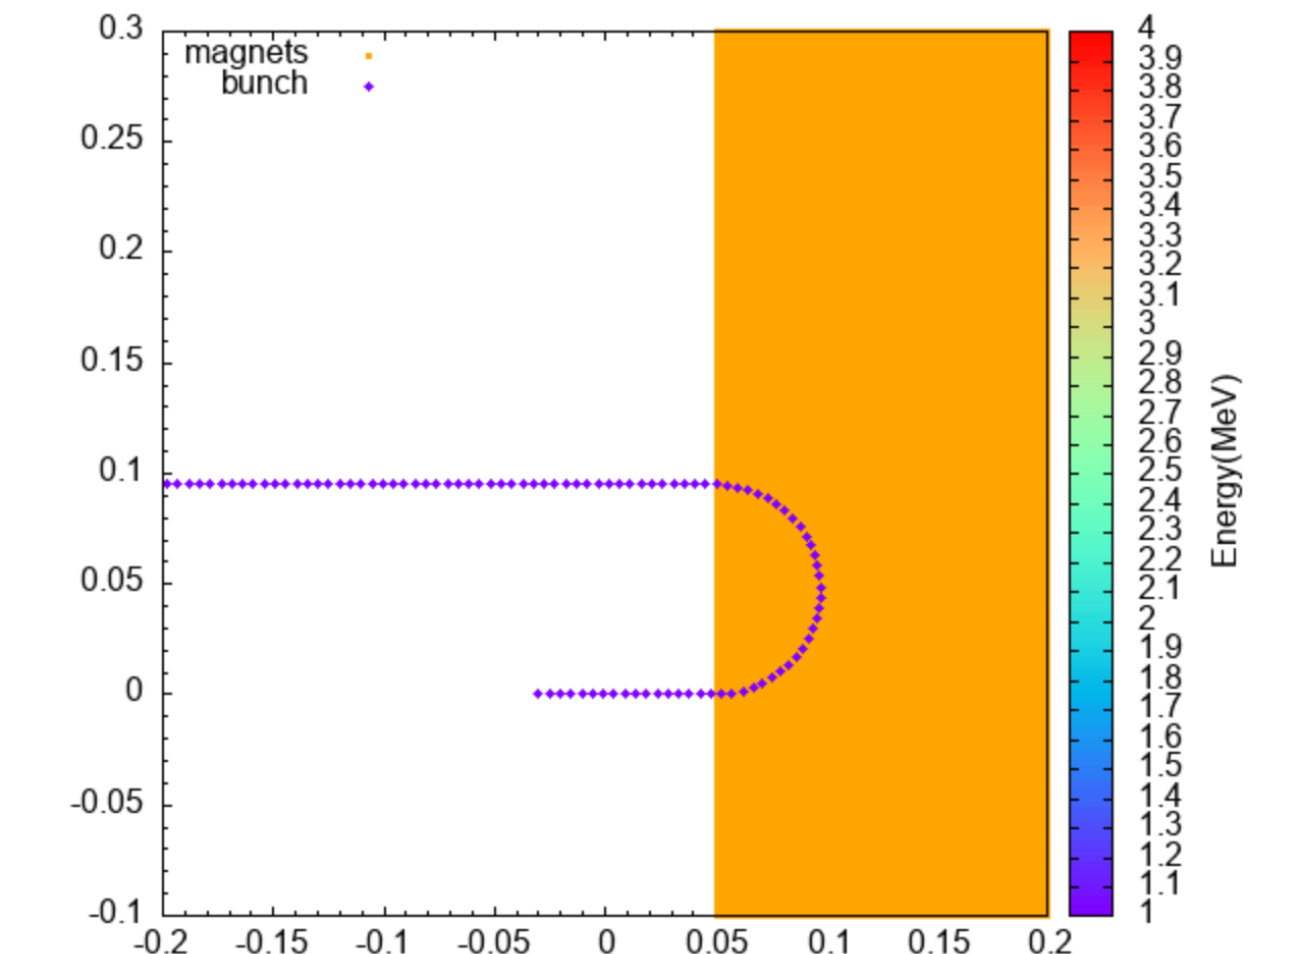
\includegraphics[width=\linewidth]{../../../figures/rhodoSim/mag_rk_00001dt.png}
        \caption*{$dt=10^{-4}$ns, $\Delta E=0.006$MeV}
    \end{subfigure}
    \caption{Energy gain of $1$MeV bunch in \textbf{B}=$0.1$T using RK4-2}
    \label{fig:mag_rk_render}
\end{figure}

\begin{figure}[H]
    \centering
    \captionsetup{justification=centering}
    \begin{minted}[linenos=true, autogobble, frame=lines, framesep=2mm, fontsize=\tiny, style=staroffice]{c++}
        #            Rhodotron Simulation Configuration File
        # ================================================================
        #    M.Furkan Er                                     22/09/2022   
        # ================================================================
        #
        # emax = Maximum electric field strength (MV/m)
        # ein = Energy of electrons coming out of the gun (MeV)
        # einstd = Standard deviation of energy of electrons coming out of the gun (MeV)
        # targeten = Max energy on the output gif (MeV)
        # freq = Frequency of the RF field (MHz)
        # phaselag = phase lag of the first electrons (degree)
        # starttime = time to start firing the gun (ns)
        # endtime = ns to run the simulation (ns)
        # dt = time interval to do the calculations (ns)
        # guntime = how long a gun pulse is (ns)
        # gunperiod = time between two gun pulses (ns)
        # enum = number of electrons to simulate in a bunch
        # bunchnum = number of times the gun fires
        # r1 = radius of the inner cylinder (m)
        # r2 = radius of the outer cylinder (m)
        # epath = path to store the electric field data
        # bpath = path to store the magnetic field data
        # cpath = path to store the settings
        # ppath = path to store electron data
        # multh = enable or disable multitheading
        # thcount = set the maximum thread to be used
        # magrotation = degrees of rotation to enter each magnet 
        # addmagnet = takes 3 input. (B , R, < Radial distance of center >)
        # output = output file name 
        
        
        # E FIELD CONFIGURATION 
        emax=1.170
        freq=107.3
        phaselag=10.0
        r1=0.1840
        r2=0.7380
        
        # B FIELD CONFIGURATION 
        magrotation=5.0
        
        # GUN CONFIGURATION 
        einmean=0.040
        einstd=0.0000
        targeten=2.0
        guntime=1.0
        gunperiod=9.3
        enum=50
        bunchnum=1
        
        # SIM CONFIGURATION 
        starttime=0
        endtime=10
        dt=0.0000010000
        epath=xy/rf.dat
        bpath=xy/magnet.dat
        cpath=xy/settings.dat
        ppath=xy/paths/
        multh=1
        thcount=10     
    \end{minted}
\caption{$\phi_{lag}$ \& $\rho$ \& $L$ optimization at \\$P=12$KW, $R_1=0.188$m, $R_2=0.753$m, $t_g=0.8$ns, $E_{in}=40$KeV}
\label{fig:config_file}
\end{figure}

\begin{figure}[H]
    \centering
    \captionsetup{justification=centering}
    \begin{minted}[linenos=true, autogobble, frame=lines, framesep=2mm, fontsize=\tiny, style=staroffice]{c++}
        -- Simulation Configuration --
        Emax : 0.96     MV/m
        Freq : 107.5    MHz
        Phase Lag : -5  degree
        EndTime : 100   ns
        dT : 0.0001     ns
        guntime : 0.8   ns
        gunperiod : 9.3 ns
        enum : 100
        bunchnum : 2
        R1 : 0.188241   m
        R2 : 0.752967   m
        Magnet count :  5
        Ein : 0.04      MeV
        TargetE : 2.5   MeV
        --------------------------------
        
                     ...Simulation is running...
        V_____________________________________________________V
        [####################################                 ]
    \end{minted}
\caption{Example of console output while simulation is running.}
\label{fig:console_output_running}
\end{figure}


\end{document}


